\documentclass[
program=itk,
%printversion,
biblatex,
language=czech,
font=sans,
figures=false,
tables=false,
theorems,
sourcecodes,
glossaries,
index
]{kidiplom}

\title{Nástroj pro tvorbu rozpočtu}
\title[english]{A Budget Creation Tool}

\author{Václav Orság}

\supervisor{Mgr. Jiří Zacpal, Ph.D.}

\yearofsubmit{\the\year}

\annotation{Cílem této bakalářské práce je vytvořit desktopovou aplikaci pro tvorbu a sledování rozpočtu. Aplikace bude zahrnovat nástroje pro vytváření a modifikaci rozpočtů, umožní uživatelům definovat vlastní účetní osnovu, a poskytne funkce pro import a export dat ve formátu CSV. Součástí aplikace budou také interaktivní grafy a reporty, které umožní sledovat plnění rozpočtu v reálném čase. Aplikace bude napsána v jazyce Python a bude navržena tak, aby byla uživatelsky přívětivá a flexibilní, což umožní široké využití v různých finančních scénářích.}

\annotation[english]{The aim of this bachelor's thesis is to develop a desktop application for budget creation and monitoring. The application will include tools for creating and modifying budgets, allow users to define their own accounting framework, and provide features for importing and exporting data in CSV format. The application will also feature interactive charts and reports to enable real-time budget tracking. It will be developed in Python and designed to be user-friendly and flexible, making it suitable for a variety of financial scenarios.}

%% Klíčová slova práce, včetně anglických. Oddělená (obvykle) středníkem.
\keywords{tvorba rozpočtu; sledování rozpočtu; desktopová aplikace; účetní osnova; import/export dat; Python}
\keywords[english]{budget creation; budget monitoring; desktop application; accounting framework; data import/export; Python}

\thanks{Děkuji vedoucímu práce Mgr. Jiřímu Zacpalovi, Ph.D. za odborné vedení, cenné rady a trpělivost při konzultacích. Dále děkuji své rodině za podporu během studia.}

\bibliography{bibliografie.bib}

%% Další dodatečné styly (balíky) potřebné pro sazbu vlastního textu
%% práce.
\usepackage{lipsum}
\usepackage{longtable}
\usepackage{graphicx}
\usepackage{subcaption}
\usepackage{float}

%% Nastavení cesty k obrázkům
\graphicspath{{obrazky/}}

\begin{document}
%% Sazba úvodních stran
\maketitle

%% Vlastní text závěrečné práce.

\section{Úvod}
Cílem této práce je navrhnout a implementovat desktopovou aplikaci pro správu osobních i firemních rozpočtů. V dnešní době je efektivní správa financí klíčová...

\section{Průzkum existujících řešení}

\subsection{EveryDollar Budgeting App}
EveryDollar je aplikace pro správu osobního rozpočtu, která uživatelům umožňuje sledovat příjmy a výdaje, nastavovat finanční cíle a plánovat úspory. Hlavním aspektem, který mne na této aplikaci zaujal, je její jednoduchost. Následující obrázky \ref{fig:planned}, \ref{fig:spent}, \ref{fig:remaining} tuto jednoduchost ilustrují. 

Na obrázku \ref{fig:planned} jsou přehledně zobrazeny všechny plánované výdaje spolu s procentuálním vyjádřením jejich podílu na celkových výdajích. Nad plánovanými výdaji se nachází graf zobrazující plánovaný příjem. Domnívám se, že by bylo užitečné, kdyby aplikace umožňovala sečíst plánované výdaje a porovnat je s grafem příjmů. V tomto případě plánované výdaje dosahují 122 \% příjmů, což výrazně překračuje náš rozpočet, avšak aplikace na tuto skutečnost neupozorňuje.

\begin{figure}[H]
    \centering
    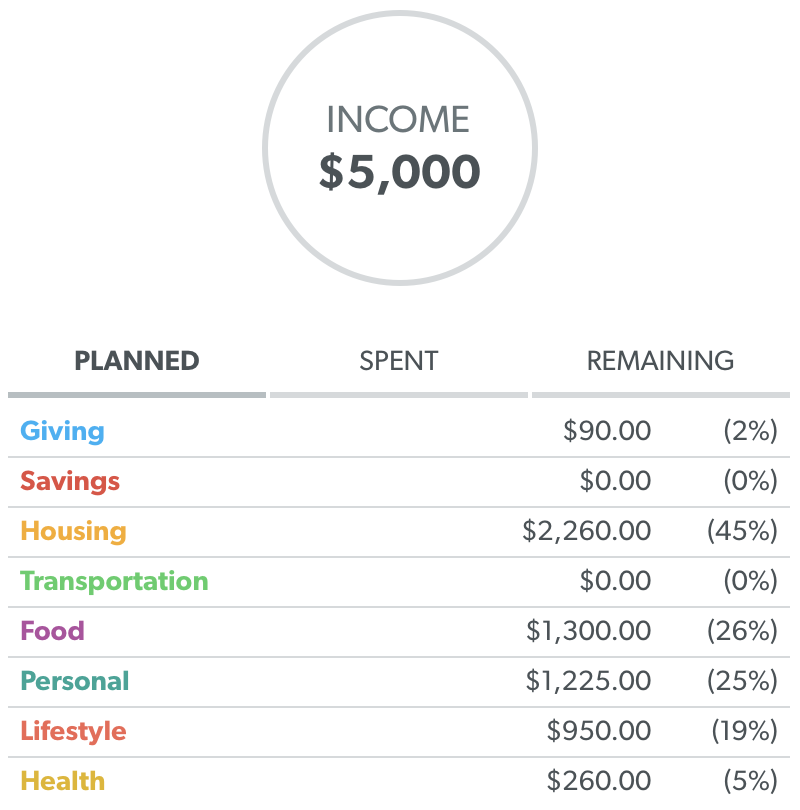
\includegraphics[width = 0.5\textwidth]{planned_income.png}
    \caption{Plánované příjmy a výdaje}
    \label{fig:planned}
\end{figure}

Obrázek \ref{fig:spent} zobrazuje skutečně vynaložené výdaje ve srovnání s plánovanými výdaji. V případě překročení plánovaného limitu se daný výdaj označí červeně, což usnadňuje identifikaci překročení rozpočtu.

\begin{figure}[H]
    \centering
    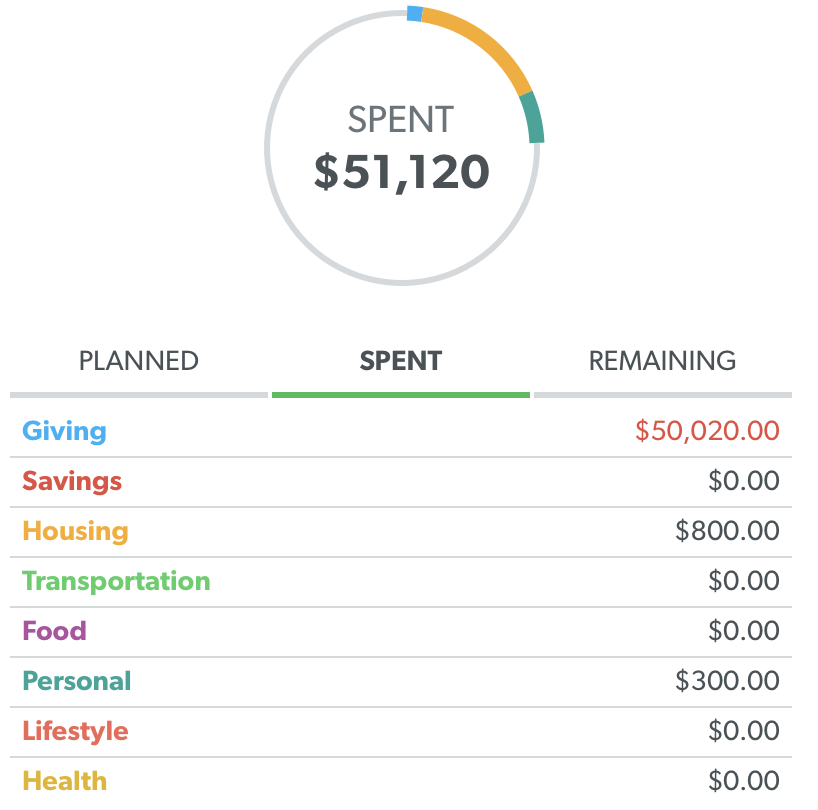
\includegraphics[width = 0.5\textwidth]{planned_income2.png}
    \caption{Porovnání plánu a skutečnosti}
    \label{fig:spent}
\end{figure}

Obrázek \ref{fig:remaining} je podle mého názoru nejvíce intuitivní. Zobrazuje zbývající část plánovaných výdajů spolu s grafickým znázorněním, což poskytuje uživatelům jasný přehled o zbývajících finančních prostředcích. 

\begin{figure}[H]
    \centering
    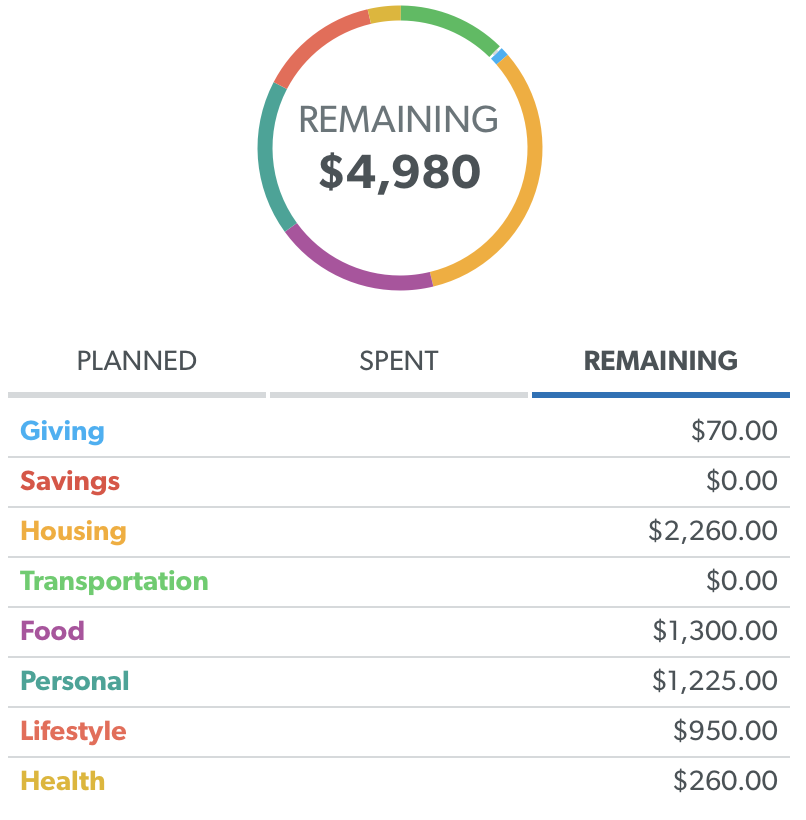
\includegraphics[width = 0.5\textwidth]{planned_income3.png}
    \caption{Zbývající prostředky}
    \label{fig:remaining}
\end{figure}

Jak jsem již zmínil při průzkumu EveryDollar Budgetting App mne zaujalo zejména grafické zpracování, které umožňuje rychlé a efektivní porozumění finanční situaci. Na základě těchto poznatků zvažuji přidání funkcionality, která by umožňovala proklik z grafu přímo na konkrétní výdaj. Tato funkcionalita by mohla dále zvýšit intuitivnost a efektivitu aplikace, což by uživatelům poskytlo rychlý přístup k detailním informacím o jejich výdajích.

\subsection{QuickBooks Accounting App}
QuickBooks je komplexní účetní a finanční aplikace, která uživatelům umožňuje efektivně spravovat jejich finanční prostředky, včetně sledování příjmů a výdajů, vystavování faktur, správy mzdových nákladů a generování finančních reportů. Co mě na této aplikaci zaujalo nejvíce, je její robustní grafické zpracování a uživatelsky přívětivé rozhraní, které poskytuje jasný a přehledný pohled na finanční situaci uživatele.

Díky intuitivnímu a vizuálně přitažlivému uspořádání dat QuickBooks umožňuje uživatelům snadno monitorovat a analyzovat jejich finanční toky. Přehledné grafy a tabulky usnadňují porozumění komplexním finančním informacím, což je klíčové pro efektivní rozhodování. 

Inspirací pro můj projekt je zejména možnost přizpůsobení hlavní stránky aplikace pomocí modifikovatelných widgetů. Zvažuji přidání podobné funkcionality, která by uživatelům umožnila personalizovat své hlavní rozhraní podle jejich specifických potřeb a preferencí.

\begin{figure}[H]
    \centering
    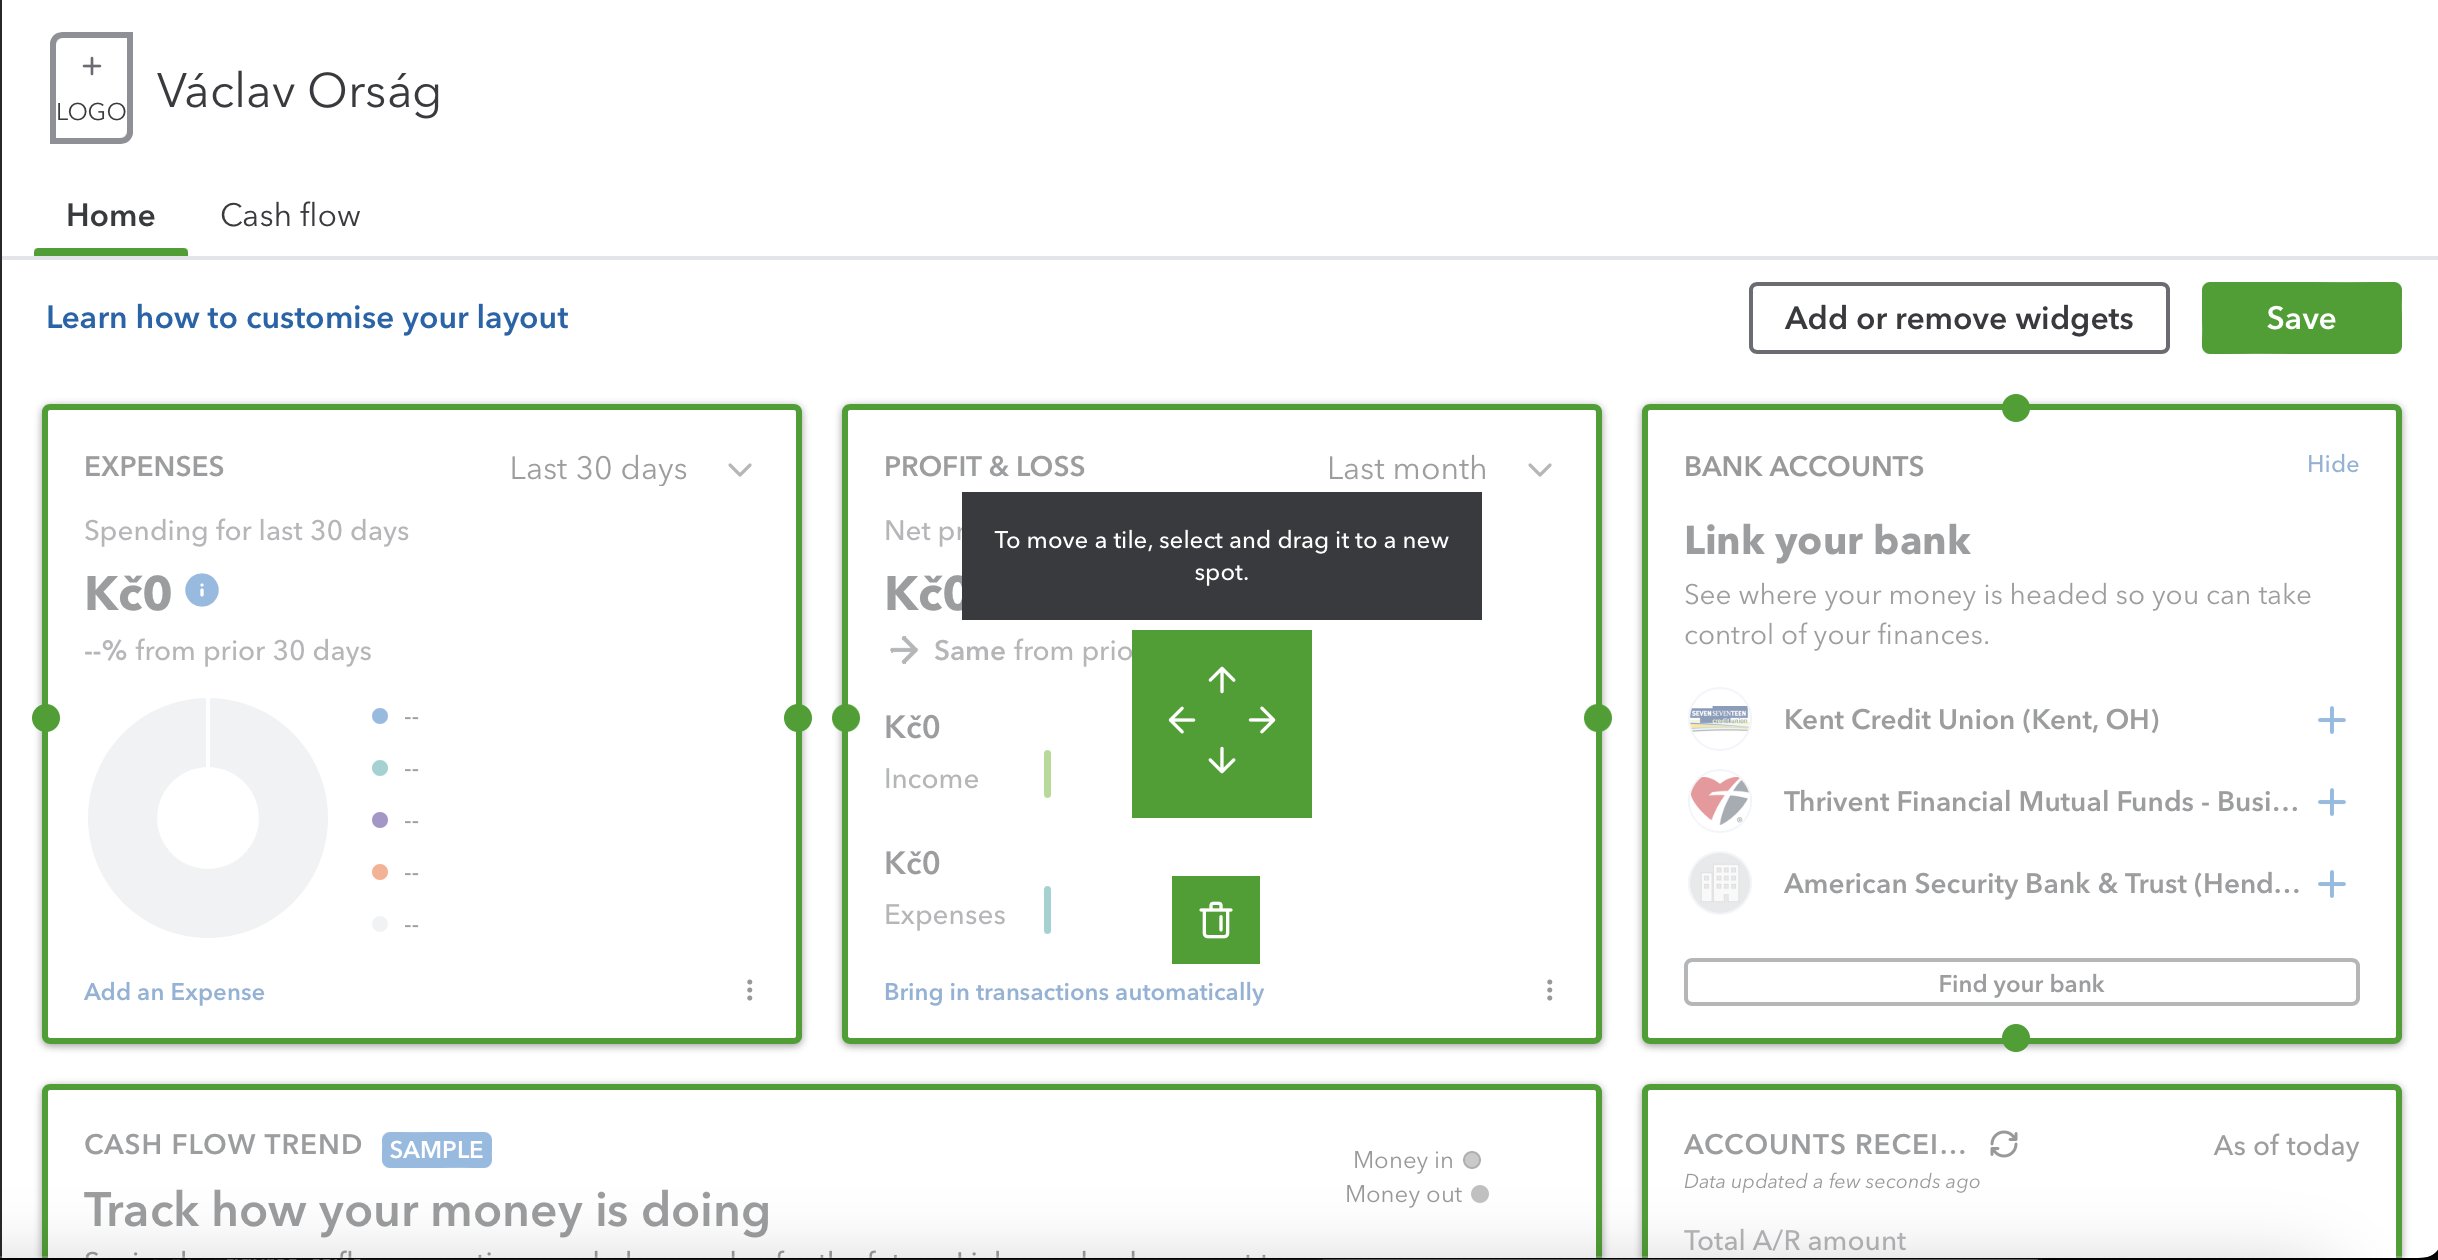
\includegraphics[width = \textwidth]{widget.png}
    \caption{Uspořádání widgetů před změnou}
    \label{fig:widget}
\end{figure}

\begin{figure}[H]
    \centering
    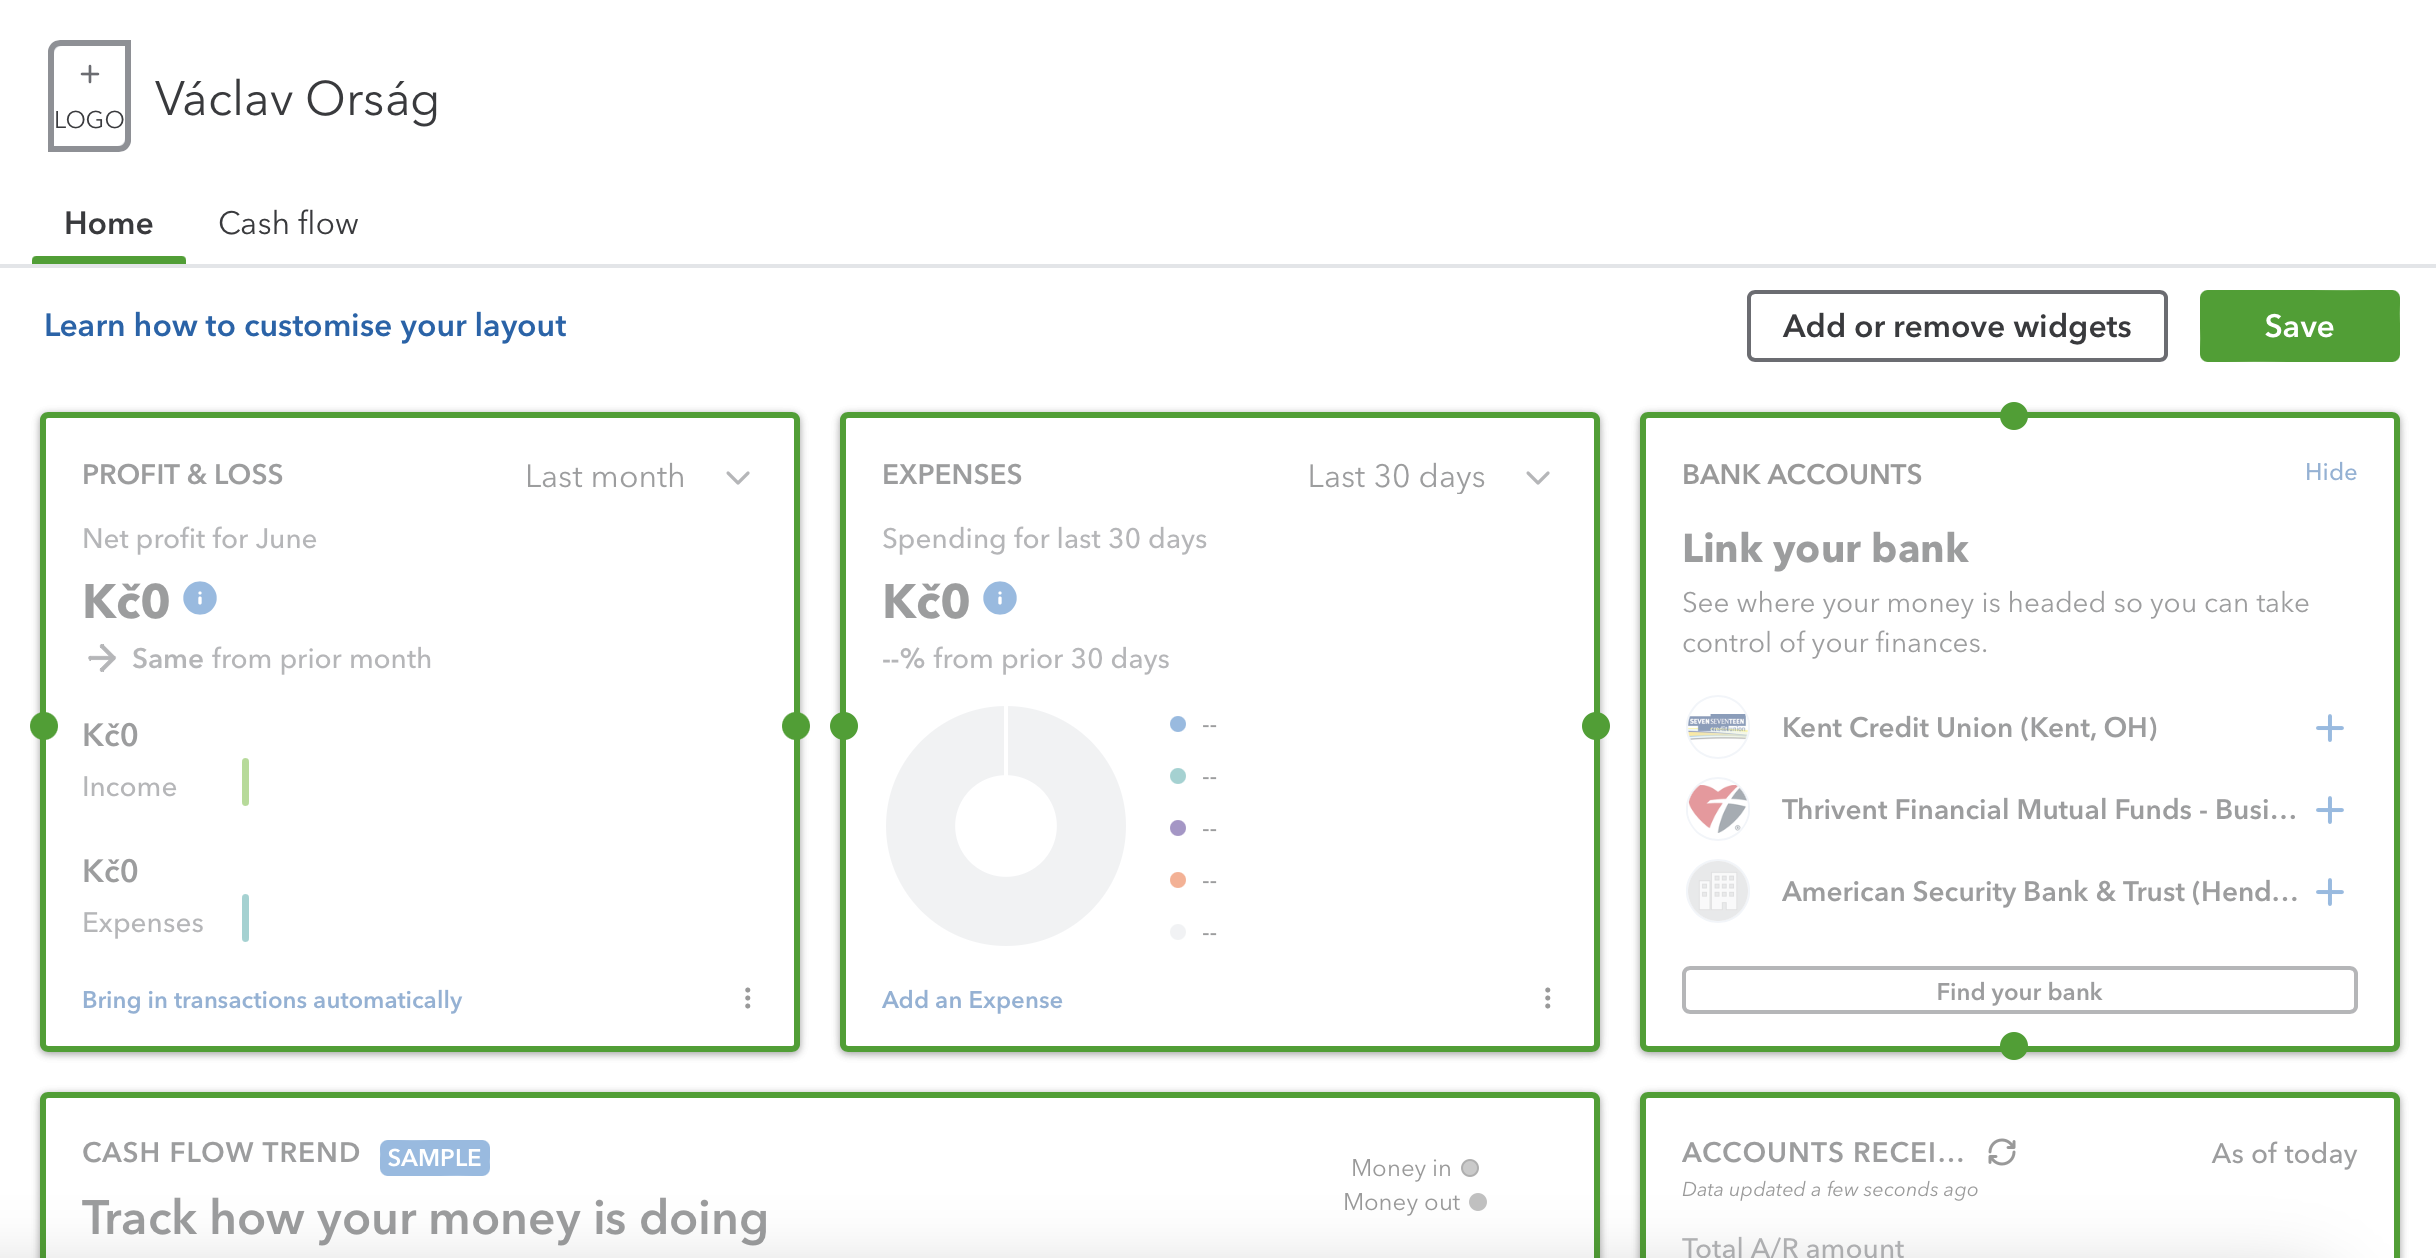
\includegraphics[width = \textwidth]{widget2.png}
    \caption{Uspořádání widgetů po změně}
    \label{fig:widget_changed}
\end{figure}

Obrázky \ref{fig:widget}, \ref{fig:widget_changed} demonstrují zmiňovanou funkcionalitu drag-and-drop. 

\subsection{Wallet by BudgetBakers}
Wallet by BudgetBakers je pokročilá aplikace pro správu osobních financí, která uživatelům poskytuje širokou škálu funkcí pro efektivní sledování a plánování jejich finančních prostředků. Umožňuje spravovat příjmy a výdaje, nastavovat finanční cíle, sledovat úspory a generovat detailní finanční reporty. Jednou z hlavních výhod Wallet je její schopnost synchronizovat data s bankovními účty uživatelů, což zajišťuje aktuálnost a přesnost finančních informací. I když tuto funkcionalitu ve své aplikaci pravděpodobně nevyužiji, slouží jako výborný nástroj pro následující demonstraci \ref{fig:report}.

Jednou z klíčových funkcí Wallet je predikce budoucích finančních toků na základě historických dat. Tato funkce umožňuje uživatelům předvídat budoucí příjmy a výdaje, což je nezbytné pro efektivní finanční plánování. Do své aplikace bych rád implementoval podobný systém reportů, který by uživatelům umožnil například srovnávat aktuální finanční situaci se stejným obdobím v minulém roce a podobně.

\begin{figure}[H]
    \centering
    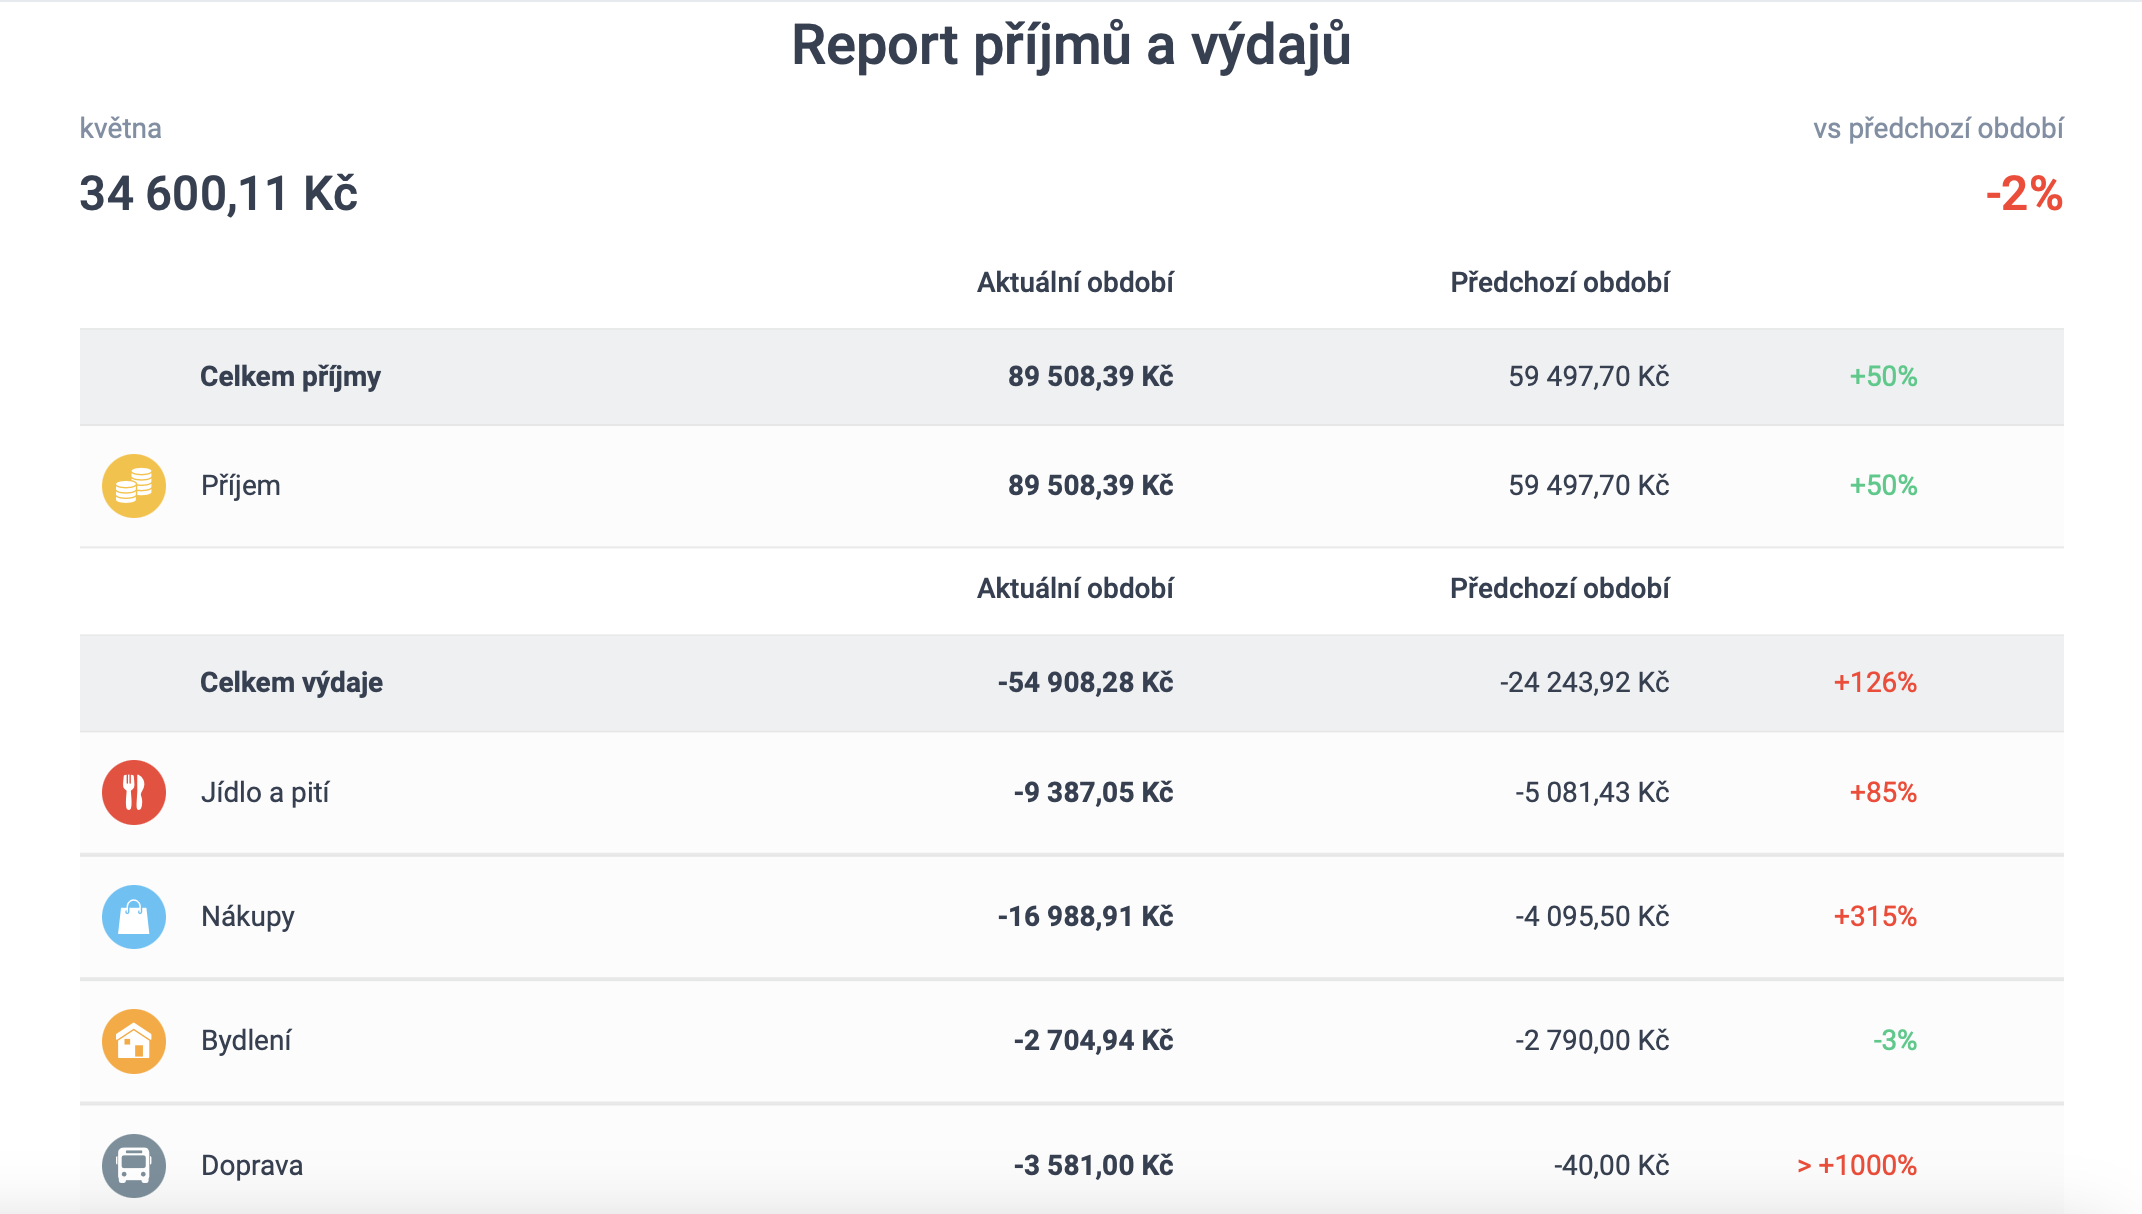
\includegraphics[width = \textwidth]{report.png}
    \caption{Reporty ve Wallet}
    \label{fig:report}
\end{figure}

\section{Specifikace řešení}

\subsection{Správa rozpočtu}
Aplikace bude obsahovat komplexní nástroje pro správu rozpočtu. Uživatelé budou moci vytvářet a modifikovat rozpočty pomocí intuitivního uživatelského rozhraní. Funkce budou zahrnovat:
\begin{itemize}
  \item Vytváření nových rozpočtů s možností nastavení různých kategorií a podkategorií.
  \item Modifikace stávajících rozpočtů, včetně přidávání, úprav a odstraňování položek.
  \item Přidávání poznámek a tagů k jednotlivým položkám rozpočtu.
\end{itemize}

\subsection{Účetní osnova}
Aplikace umožní uživatelům vytvořit a spravovat vlastní účetní osnovu, která bude plně konfigurovatelná. Hlavní funkce zahrnují:
\begin{itemize}
  \item Vytváření nových účetních osnov s možností přidávání kategorií a podkategorií.
  \item Úprava stávajících účetních osnov, včetně možnosti měnit strukturu a hierarchii.
  \item Přidávání popisů a tagů k jednotlivým položkám v účetní osnově pro lepší přehlednost a organizaci.
\end{itemize}

\subsection{Import a export dat}
Aplikace bude podporovat import a export dat ve formátu CSV, což umožní snadný přenos dat mezi různými zařízeními a aplikacemi. Funkce budou zahrnovat:
\begin{itemize}
  \item Import dat z CSV souborů, což umožní uživatelům rychle načíst data do aplikace a zároveň bude dopomáhat k automatickému vytvoření předběžného rozpočtu. 
  \item Export dat do CSV souborů, což umožní uživatelům snadno zálohovat a sdílet svá data.
  \item Pro import a export dat z textových souborů je vhodné použít modul CSV v Pythonu nebo knihovnu Pandas pro pokročilejší manipulaci s daty. Modul CSV umožňuje snadný import a export dat z textových souborů, zatímco Pandas nabízí výkonné nástroje pro analýzu a zpracování dat.
\end{itemize}

\subsection{Sledování plnění rozpočtu}
Aplikace nabídne nástroje pro interaktivní sledování plnění rozpočtu. Uživatelé budou moci sledovat své finanční cíle a analyzovat data pomocí grafů a reportů. Hlavní funkce budou zahrnovat:
\begin{itemize}
  \item Grafické zobrazení plnění rozpočtu v reálném čase.
  \item Tvorbu reportů, které poskytují detailní přehled o příjmech a výdajích.
  \item Možnost nastavení finančních cílů a sledování jejich plnění.
  \item Analýza trendů a vzorců ve financích uživatele pomocí interaktivních nástrojů.
\end{itemize}

\subsection{Grafy a reporty}
Pro vizualizaci dat a tvorbu grafů je vhodné použít knihovnu Matplotlib. Matplotlib nabízí širokou škálu možností pro tvorbu grafů a je dobře integrovatelný s Pythonem a Tkinterem.

\section{Použité technologie}

\subsection{Programovací jazyk a framework}
Pro vývoj desktopové aplikace je ideální volbou programovací jazyk Python v kombinaci s GUI toolkitem Tkinter. Python je známý svou jednoduchostí a čitelností, což usnadňuje vývoj a údržbu aplikace. Tkinter je základní GUI toolkit pro Python, který umožňuje vytvářet plně funkční desktopové aplikace.

\subsection{Databáze}
Pro ukládání dat je vhodná databáze SQLite. SQLite je lehká databáze, která nevyžaduje samostatný server a umožňuje ukládání dat přímo do souboru. To je ideální pro desktopové aplikace, kde je potřeba jednoduché a efektivní řešení pro správu dat.

\section{Programátorská příručka}
Tato kapitola bude popisovat samotný vývoj aplikace, strukturu kódu a řešení klíčových problémů...

\section{Uživatelská příručka}

Tato kapitola slouží jako průvodce pro uživatele aplikace. Popisuje instalaci, spuštění a základní scénáře použití.

\subsection{Spuštění aplikace}
Aplikace nevyžaduje složitou instalaci. Pro spuštění stačí otevřít soubor \texttt{main.py} (nebo spustit vygenerovaný .exe soubor). Po spuštění se zobrazí uvítací okno aplikace (viz Obrázek \ref{fig:welcome_window}). 
Zde je možné vybrat si mezi vytvořením nového rozpočtu nebo načtením existujícího.

\begin{figure}[H]
    \centering
    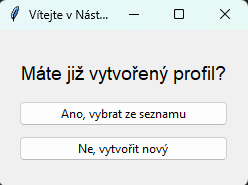
\includegraphics[width=0.8\textwidth]{welcome_window.png}
    \caption{Uvítací okno aplikace}
    \label{fig:welcome_window}
\end{figure}

Pokud profil máme zvolíme možnost : Ano, vybrat  ze seznamu a zobrazí se nám okno (viz Obrázek \ref{fig:profiles}). 
Zde si můžeme zvolit svůj existující profil ze seznamu a kliknout na tlačítko "otevřít vybraný", tím profil načteme a přesuneme se do hlavního okna aplikace (viz Obrázek \ref{fig:main_window_step_1}).
Případně se můžeme vrátit zpět na uvítací obrazovku kliknutím na tlačítko "Zpět".

\begin{figure}[H]
    \centering
    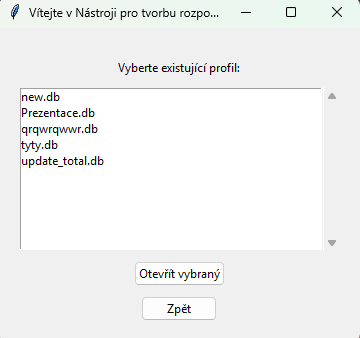
\includegraphics[width=1\textwidth]{profiles.png}
    \caption{Výběr profilu}
    \label{fig:profiles}
\end{figure}

Pokud profil nemáme zvolíme možnost : Ne, vytvořit nový a zobrazí se nám okno (viz Obrázek \ref{fig:create_new}). 
Zde je možné pojmenovat si svůj profil a kliknout na tlačítko uložit, tím profil vytvoříme a přesuneme se do hlavního okna aplikace (viz Obrázek \ref{fig:main_window_step_1}).

\begin{figure}[H]
    \centering
    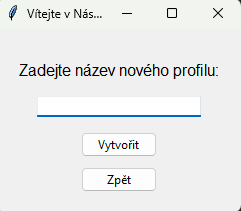
\includegraphics[width=1\textwidth]{create_new.png}
    \caption{Vytvoření nového profilu}
    \label{fig:create_new}
\end{figure}

\begin{figure}[H]
    \centering
    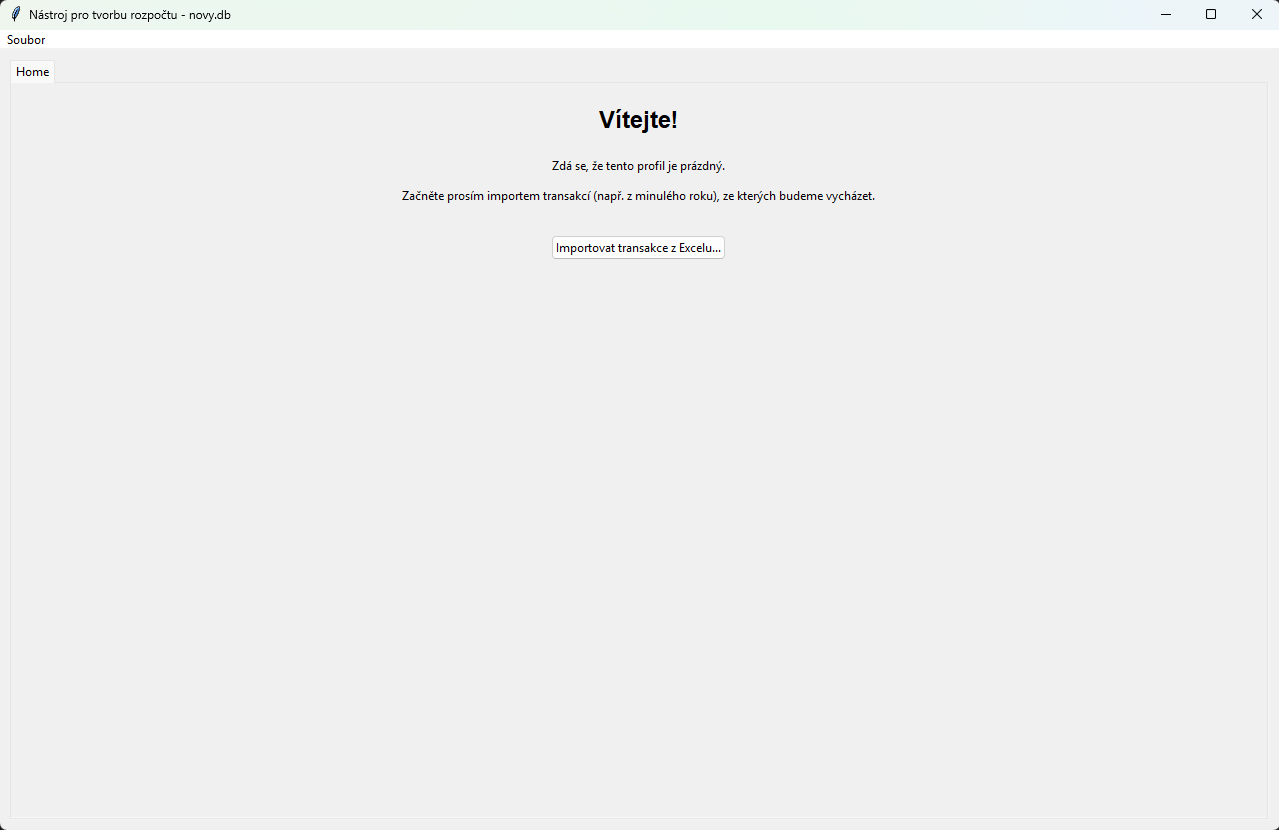
\includegraphics[width=1\textwidth]{main_window_step_1.png}
    \caption{Hlavní okno aplikace}
    \label{fig:main_window_step_1}
\end{figure}





\subsection{Importování transakcí z excelu}
Po vytvoření nového profilu se uživateli zobrazí hlavní okno aplikace (viz Obrázek \ref{fig:main_window_step_1}). Zde má zatím uživatel většinu funkcionalit uzamčených. 
Pro odemčení funkcí je potřeba projít "tutoriálem", který se postupně vždy aktualizuje v záložce Home. (Aktuálně jediné viditelné záložce.)

Pro importování transakcí je potřeba mít připravený excelový soubor, který obsahuje list s názvem "Zdroj". Tento list musí obsahovat sloupce: Datum, Doklad, Zdroj, Firma, Text, MD, D, částka, Cin, číslo, Co, Kdo, Středisko.
Po kliknutí na tlačítko "Importovat transakce z Excelu" se zobrazí dialogové okno (viz Obrázek \ref{fig:choose_window}) pro výběr souboru. 
Uživatel vybere svůj excelový soubor a klikne na tlačítko "Otevřít". Aplikace si načte data z vybraného souboru a zobrazí potvrzení importu (viz Obrázek \ref{fig:import_confirm}).
Zároveň se aktualizuje Home záložka s informací o úspěšném importu a dalším krokem v tutoriálu a zviditelní se nám nové záložky: Transakce a účetní osnova. (viz Obrázek \ref{fig:main_window_step_2})
\begin{figure}[H]
    \centering
    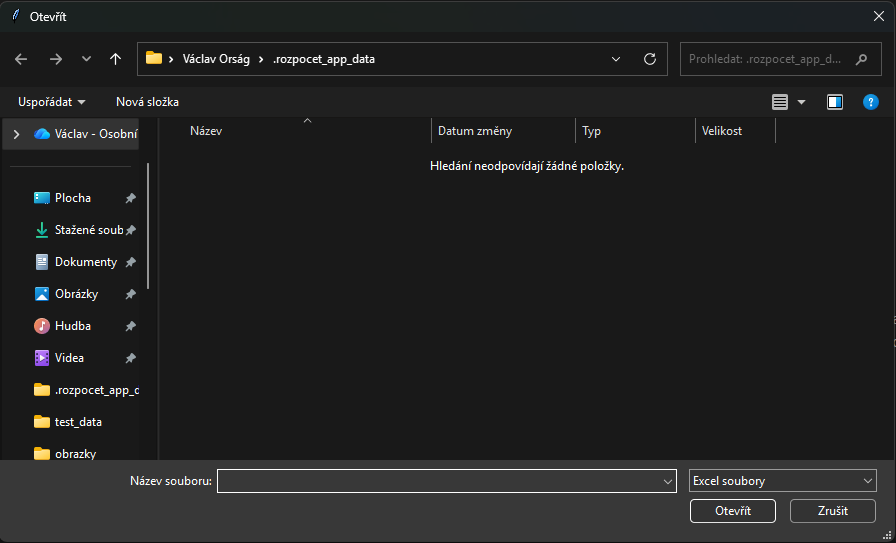
\includegraphics[width=1\textwidth]{choose_window.png}
    \caption{Výběr souboru pro import}
    \label{fig:choose_window}
\end{figure}
\begin{figure}[H]
    \centering
    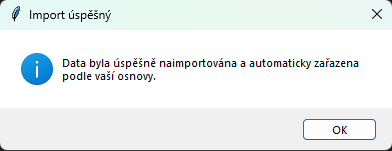
\includegraphics[width=0.8\textwidth]{import_confirm.png}
    \caption{Potvrzení importu}
    \label{fig:import_confirm}
\end{figure}


\subsection{Tvorba osnovy}
Po úspěšném importu transakcí se uživateli v Home záložce zobrazí další krok tutoriálu (viz Obrázek \ref{fig:main_window_step_2}).
Pro vytvoření osnovy je potřeba kliknout na tlačítko "Přejít na tvorbu osnovy" (Případně na záložku: účetní osnova). Tím se uživatel přesune do záložky "účetní osnova" (viz Obrázek \ref{fig:chart_tab}).

\begin{figure}[H]
    \centering
    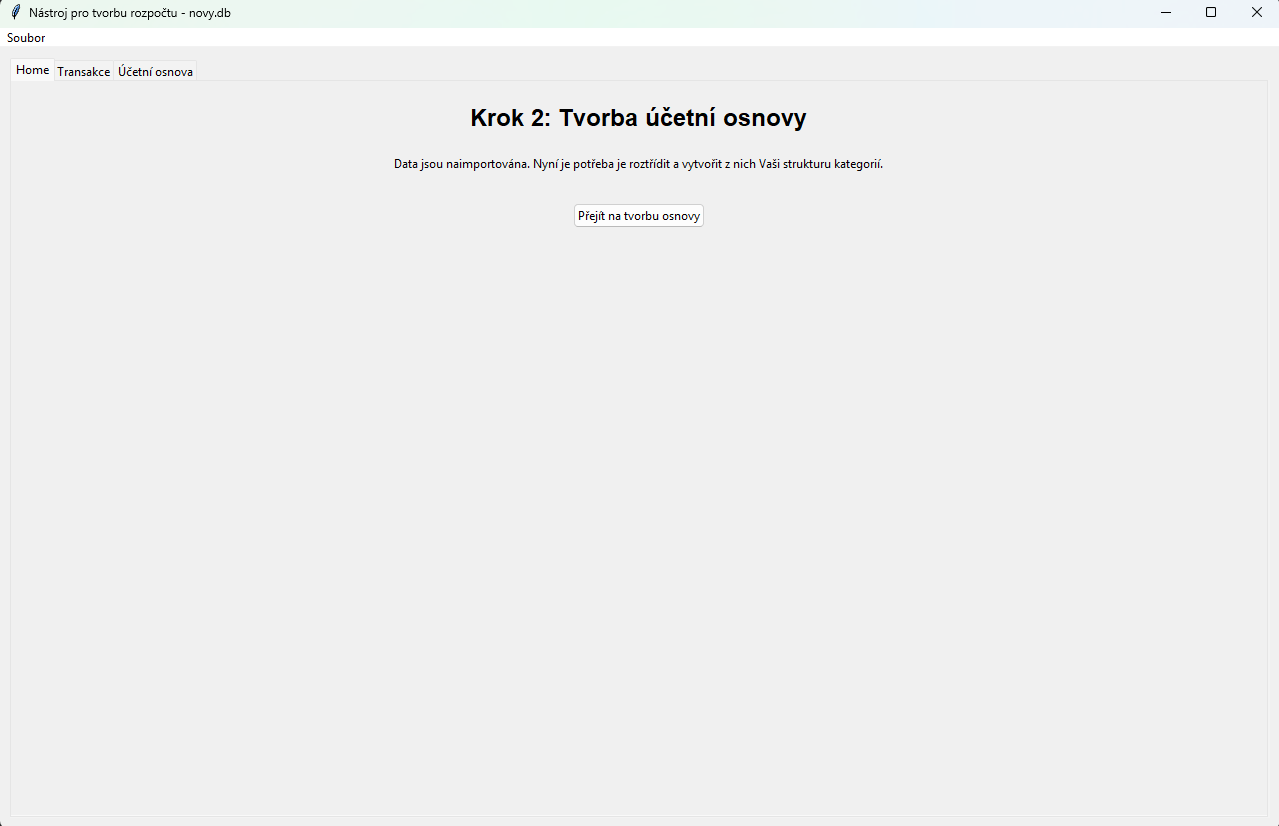
\includegraphics[width=1\textwidth]{main_window_step_2.png}
    \caption{Home tab po importu}
    \label{fig:main_window_step_2}
\end{figure}

\begin{figure}[H]
    \centering
    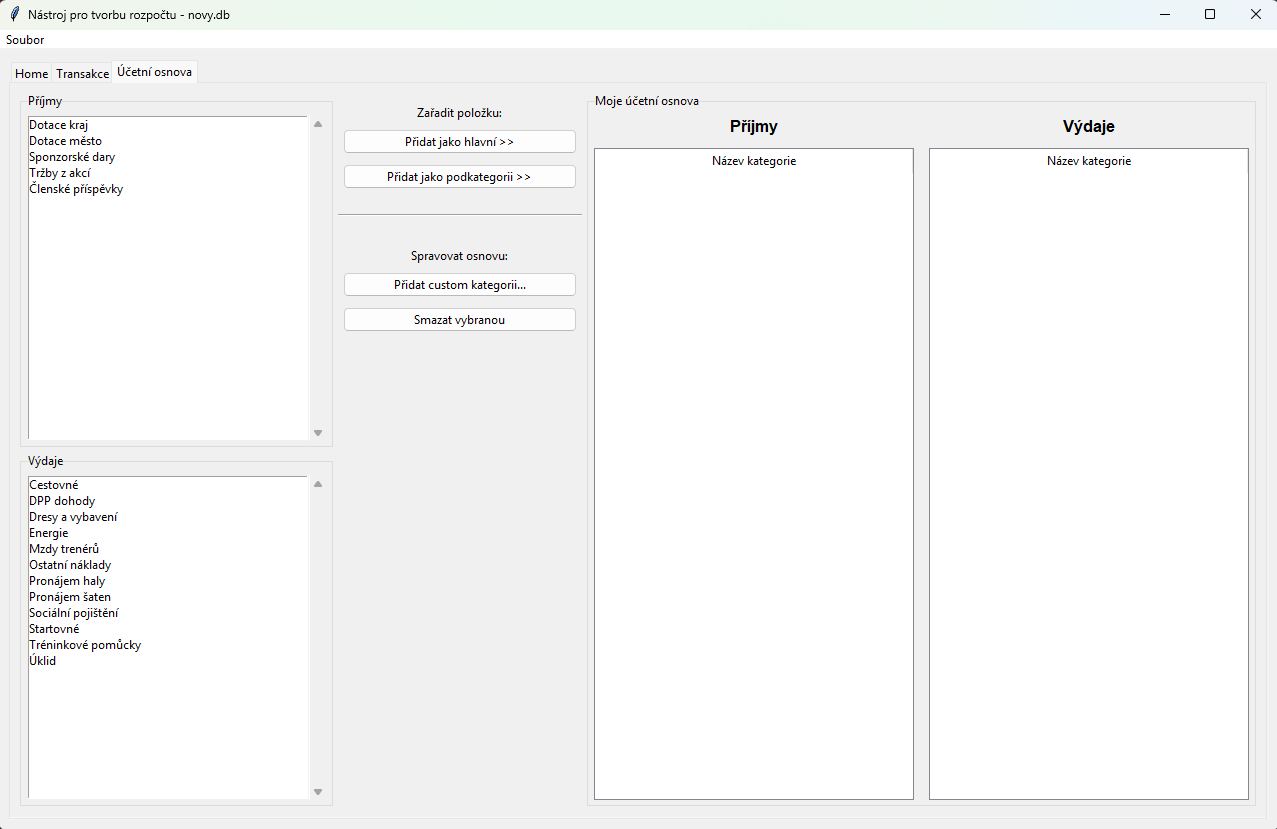
\includegraphics[width=1\textwidth]{chart_tab.png}
    \caption{Tab účetní osnova}
    \label{fig:chart_tab}
\end{figure}

Zde si uživatel může vytvořit vlastní účetní osnovu. Hlavní je logika \textbf{transakčních} vs \textbf{custom} kategorií. Transakční kategorie jsou ty, které jsou přímo spojené s importovanými transakcemi z excelu.
Custom kategorie jsou ty, které si uživatel vytvoří sám pro lepší přehlednost a organizaci (těmto kategoriím nikdy nebudou přiřazeny žádné transakce).
Aplikace sama analyzuje data na základě historických a aktuálních transakcí a jednotlivé transakce rozděluje do kategorii podle hodnoty ve sloupci "Co" v excelu, zároveň automaticky určuje typ
kategorie (MD/D) na základě hodnoty ve sloupci "MD" a "D" v excelu.

\subsubsection{Přidání hlavních kategorií}
Pokud žádnou kategorii v účetní osnově nemáme, musíme přidat \textbf{hlavní kategorii}, tou může být buď kategorie z příjmů/výdajů nebo naše custom kategorie. Pokud chceme přidat kategorii z příjmů/výdajů, 
klikneme na danou kategorii v seznamu a na tlačítko \textbf{Přidat jako hlavní}. Pokud chceme přidat custom kategorii klikneme na \textbf{Přidat custom kategorii}, je potřeba nejdříve vyplnit název kategorie
 (viz Obrázek \ref{fig:custom_category}) a poté typ (viz Obrázek \ref{fig:category_type}).
\begin{figure}[H]
    \centering
    
\includegraphics[width=0.5\textwidth]{custom_category.png}
    \caption{Volba jména custom kategorie}
    \label{fig:custom_category}
\end{figure}
\begin{figure}[H]
    \centering
    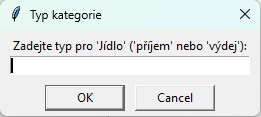
\includegraphics[width=0.5\textwidth]{category_type.png}
    \caption{Volba typu custom kategorie}
    \label{fig:category_type}
\end{figure}
Custom kategorie se zobrazují odlišně od transakčních, jsou červené a mají u sebe ikonu složky (viz Obrázek \ref{fig:custom_category_look}).
\begin{figure}[H]
    \centering
    
\includegraphics[width=0.5\textwidth]{custom_category_look.png}
    \caption{Vzhled custom kategorie v účetní osnově}
    \label{fig:custom_category_look}
\end{figure}
Poté co přidáme jakoukoliv první hlavní kategorii, se nám zobrazí upozornění, že rozpočet je připraven k použití (viz Obrázek \ref{fig:budget_ready}) a odemkne se nám nová záložka \textbf{Rozpočet}.
\begin{figure}[H]
    \centering
    
\includegraphics[width=1\textwidth]{budget_ready.png}
    \caption{Upozornění, že rozpočet je připraven k použití}
    \label{fig:budget_ready}
\end{figure}
\subsubsection{Přidání podkategorií}
Pokud jsme vytvořili custom kategorii, tak teď můžeme začít přidávat i podkategorie. Podkategorie můžeme přidávat pouze pod custom kategorie. Hlavní kategorie se samy řadí do sekcí příjmů a výdajů na základě typu.
Ale podkategorie a custom kategorie už musíme řadit ručně. Pro přidání podkategorie je potřeba vybrat kategorii, kterou chceme zařadit jako podkategorii a hlavní kategorii v seznamu účetní osnovy a kliknout na tlačítko 
\textbf{Přidat jako podkategorii} (viz Obrázek \ref{fig:add_sub_1} a \ref{fig:add_sub_2}).
\begin{figure}[H]
    \centering
    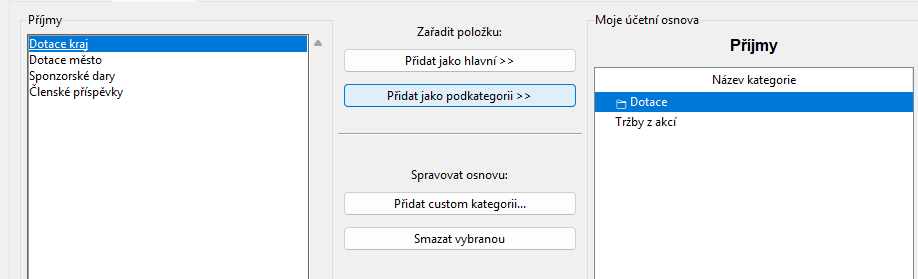
\includegraphics[width=1\textwidth]{add_sub_1.png}
    \caption{Přidání podkategorie - krok 1}
    \label{fig:add_sub_1}
\end{figure}
\begin{figure}[H]
    \centering
    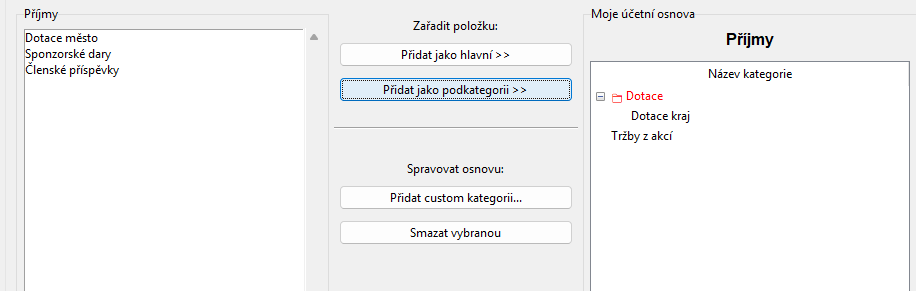
\includegraphics[width=1\textwidth]{add_sub_2.png}
    \caption{Přidání podkategorie - krok 2}
    \label{fig:add_sub_2}
\end{figure}
Pokud uděláme chybu a přidáme kategorii špatně, můžeme ji jednoduše odstranit tlačítkem \textbf{Smazat vybranou}, mazat můžeme, ale pouze kategorie, které nemají podkategorie.

Po vytvoření může osnova vypadat například takto (viz Obrázek \ref{fig:final_chart}).
\begin{figure}[H]
    \centering
    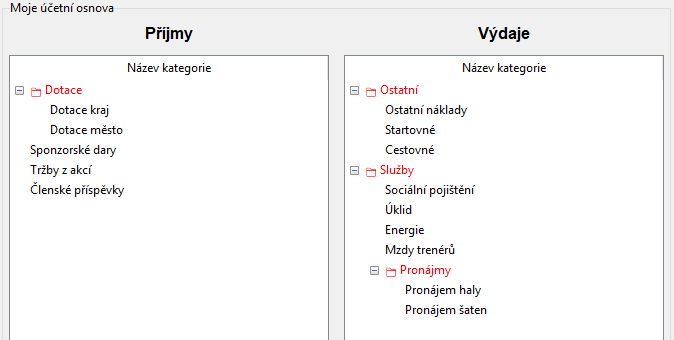
\includegraphics[width=1\textwidth]{final_chart.png}
    \caption{Finální podoba účetní osnovy}
    \label{fig:final_chart}
\end{figure}


\subsection{Tvorba rozpočtu}
Po vytvoření účetní osnovy se uživateli v Home záložce zobrazí další krok tutoriálu (viz Obrázek \ref{fig:main_window_step_3}).
\begin{figure}[H]
    \centering
    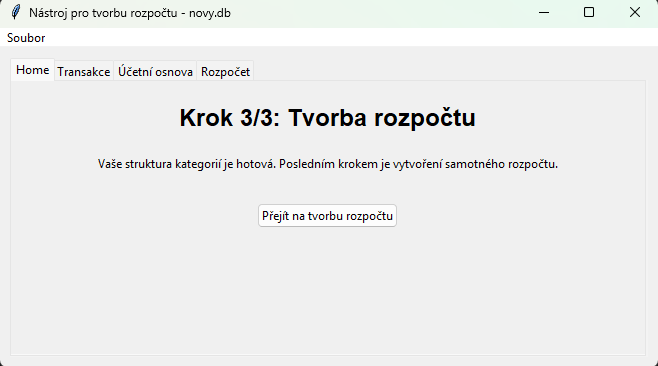
\includegraphics[width=1\textwidth]{main_window_step_3.png}
    \caption{Home tab po vytvoření účetní osnovy}
    \label{fig:main_window_step_3}  
\end{figure}
Pro vytvoření rozpočtu je potřeba kliknout na tlačítko \textbf{Přejít na tvorbu rozpočtu} (Případně na záložku: Rozpočet). Tím se uživatel přesune do záložky \textbf{Rozpočet} 

První(prázdný) rozpočet bude vypadat takto v zavislosti na osnově: (viz Obrázek \ref{fig:empty_budget_tab}).
\begin{figure}[H]
    \centering
    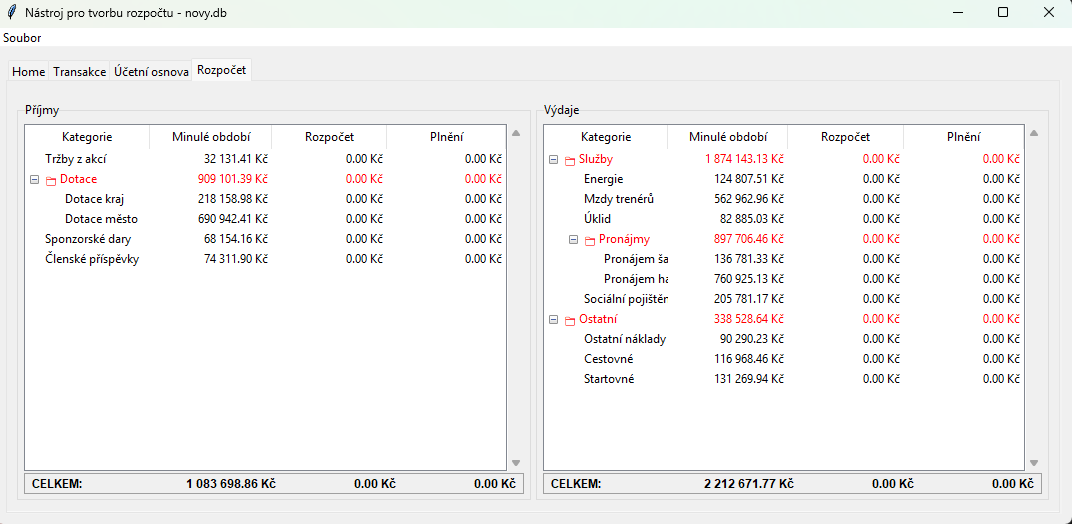
\includegraphics[width=1\textwidth]{empty_budget_tab.png}
    \caption{Tab rozpočet před vytvořením rozpočtu}
    \label{fig:empty_budget_tab}
\end{figure}

Vidíme 2 hlavní sekce - příjmy a výdaje, které odpovídají naší účetní osnově. Tyto sekce jsou rozděleny 4 sloupce, první sloupec \textbf{kategorie} zobrazuje hierarchii dle naši účetní osnovy, druhý sloupec \textbf{minulé období}
je součet všech transakcí v dané kategorii z minulých transakcí (z excelu), třetí sloupec je \textbf{rozpočet} zde budeme editovat plánované rozpočty pro jednotlivé kategorie a čtvrtý sloupec je \textbf{plnění}, zde se zobrazuje
aktuální stav plnění rozpočtu na základě importovaných aktualních transakcí.

\subsubsection{Nastavení rozpočtu}
Pro nastavení rozpočtu dané kategorie je potřeba dvojkliknout na buňku ve sloupci rozpočet na řádku dané kategorie (viz Obrázek \ref{fig:edit_budget_1}) zadat chtěnou částku 
a potvrdit klávesou Enter(viz Obrázek \ref{fig:edit_budget_2})
\begin{figure}[H]
    \centering
    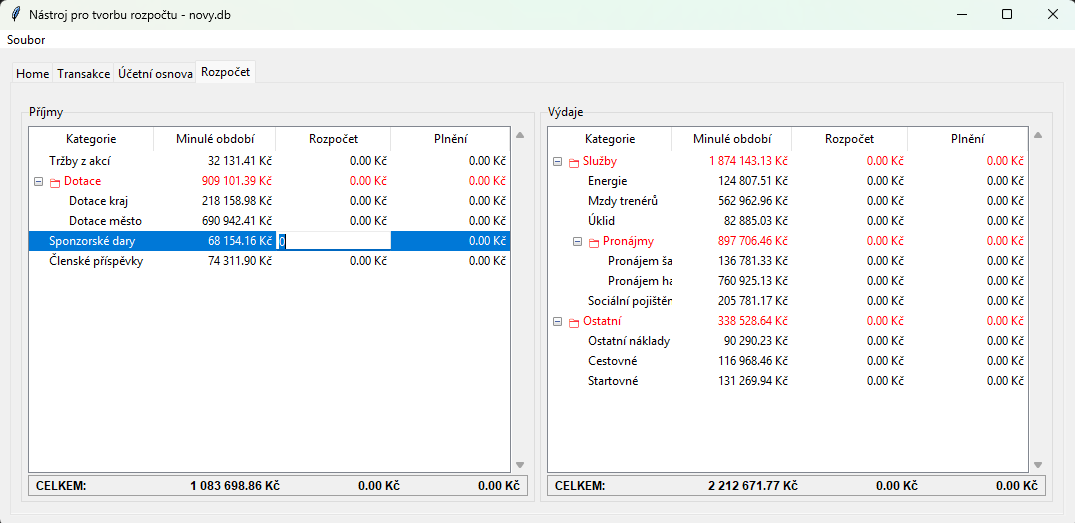
\includegraphics[width=1\textwidth]{edit_budget_1.png}
    \caption{Úprava rozpočtu - krok 1}
    \label{fig:edit_budget_1}
\end{figure}
\begin{figure}[H]
    \centering
    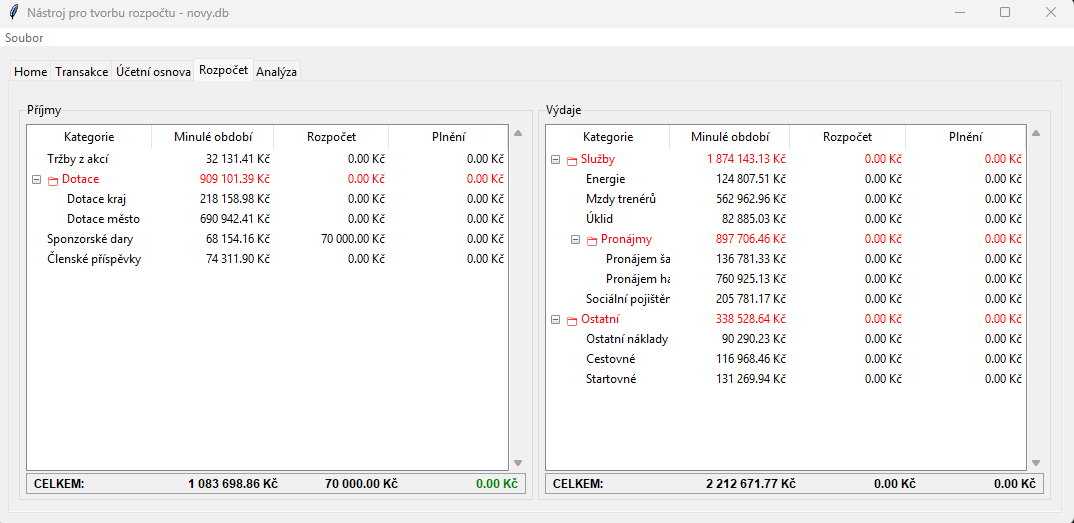
\includegraphics[width=1\textwidth]{edit_budget_2.png}
    \caption{Úprava rozpočtu - krok 2}
    \label{fig:edit_budget_2}
\end{figure}

Pokud jsme vložili úplně první rozpočet, tak se nám zobrazí nová záložka \textbf{Analýza}, aplikace nás upozorní vyskakovacím oknem (viz Obrázek \ref{fig:first_budget_info}) 
a navrhne nám import aktuálních dat, které zpřístupní záložku Plnění a umožní analyzovat aktualní data.
\begin{figure}[H]
    \centering
    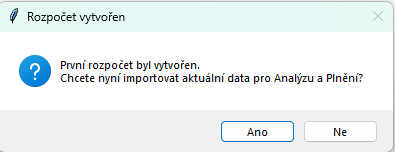
\includegraphics[width=0.8\textwidth]{first_budget_info.png}
    \caption{Informace o vytvoření prvního rozpočtu}
    \label{fig:first_budget_info}
\end{figure}

Data můžeme importovat kliknutím na Ano tím se zobrazí dialogové okno pro výběr dat k importu (viz Obrázek \ref{fig:import_current}). Pro import je potřeba mít připravený excelový soubor, 
který obsahuje list s názvem \textbf{Zdroj}. Tento list musí obsahovat sloupce: \textbf{Datum, Doklad, Zdroj, Firma, Text, MD, D, částka, Cin, číslo, Co, Kdo, Středisko}.
\begin{figure}[H]
    \centering
    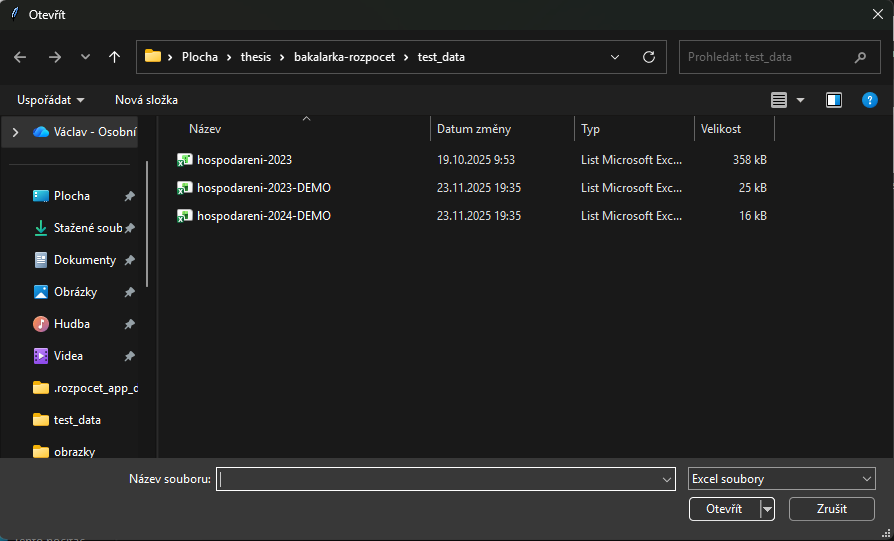
\includegraphics[width=0.8\textwidth]{import_current.png}
    \caption{Import aktuálních dat}
    \label{fig:import_current}
\end{figure}
Pokud jsme data neimportovali, můžeme tak učinit později v záložce \textbf{Home}. Zde se zobrazí další krok tutoriálu 
(viz Obrázek \ref{fig:main_window_step_4}). 
\begin{figure}[H]
    \centering
    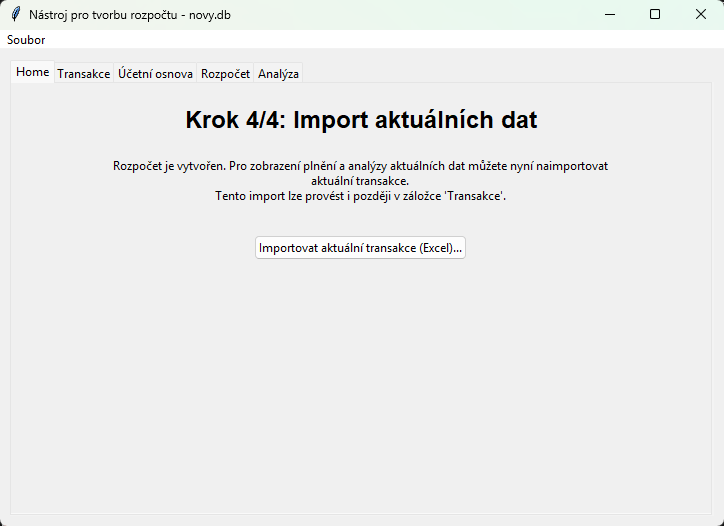
\includegraphics[width=1\textwidth]{main_window_step_4.png}
    \caption{Home tab po vytvoření prvního rozpočtu}
    \label{fig:main_window_step_4}
\end{figure}
Kliknutím na tlačítko \textbf{Importovat aktuální data} se zobrazí dialogové okno pro výběr souboru (viz Obrázek \ref{fig:import_current}).

Po úspěšném importu se nám zobrazí potvrzení importu (viz Obrázek \ref{fig:import_current_confirm}).
\begin{figure}[H]
    \centering
    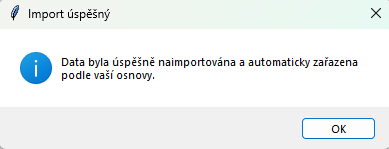
\includegraphics[width=0.8\textwidth]{import_current_confirm.png}
    \caption{Potvrzení importu aktuálních dat}
    \label{fig:import_current_confirm}
\end{figure}
Zároveň se aktualizuje záložka \textbf{Home}, ze které se teď stává tzv. \textbf{Dashboard}, v záložce \textbf{Analýza} teď můžeme analyzovat i aktuální data a v záložce \textbf{Transakce} můžeme pracovat s aktuálními transakcemi.
  

\subsection{Analýza transakcí}
Záložka \textbf{Analýza} nám umožňuje dynamicky seskupovat transakce pomocí hierarchického pohledu (tzv. pivot table) a sledovat součty na jednotlivých úrovních. Můžeme přepínat mezi jednotlivými presety, 
zobrazovat historické nebo aktuální transakce a filtrovat, jestli chceme zobrazit pouze výdaje, příjmy nebo obojí.

Celou analýzu ovládáme pomocí panelu nástrojů v horní části záložky (viz Obrázek \ref{fig:analysis_toolbar}).
\begin{figure}[H]
    \centering
    
\includegraphics[width=1\textwidth]{analysis_toolbar.png}
    \caption{Panel nástrojů v záložce Analýza}
    \label{fig:analysis_toolbar}
\end{figure}
Funkce \textbf{řádky} je ve výchozím nastavení zašedlá a nelze na ni kliknout, protože hierarchie je nastavena podle výchozího presetu. O změně hierarchie se dozvíme v sekci Presety.
\subsubsection{Hierarchický pohled}
V záložce \textbf{Analýza} vidíme hierarchický pohled na naše transakce (viz Obrázek \ref{fig:analysis_tab}). Ve výchozím nastavení je hierarchie nastavena podle presetu \textbf{Analýza středisek}, 
ale uživatel může tuto hierarchii měnit podle svých potřeb (viz sekce Presety).
\begin{figure}[H]
    \centering
    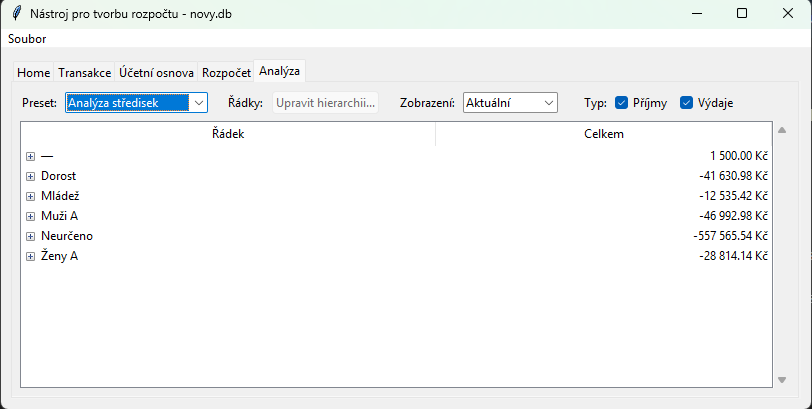
\includegraphics[width=1\textwidth]{analysis_tab.png}
    \caption{Tab Analýza}
    \label{fig:analysis_tab}
\end{figure}
Na obrázku \ref{fig:analysis_tab} vidíme 2 hlavní sloupce - \textbf{řádek} a \textbf{Celkem}, kde řádek zobrazuje naši nastavenou hierarchii a celkem zobrazuje součet všech transakcí odpovídající danému řádku. 
Hierarchii můžeme rozbalovat a sbalovat kliknutím na ikony + a - vlevo od řádku (viz Obrázek \ref{fig:analysis_expand}). Můžeme tak docílit detailního pohledu na naše transakce.
\begin{figure}[H]
    \centering
    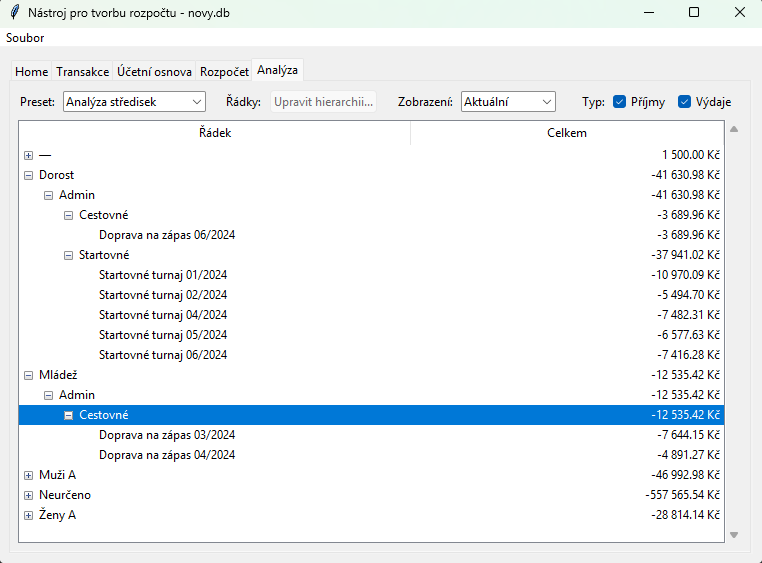
\includegraphics[width=1\textwidth]{analysis_expand.png}
    \caption{Rozbalení a sbalení hierarchie}
    \label{fig:analysis_expand}
\end{figure}
\subsubsection{Presety}
Presety nám umožňují rychle měnit hierarchii zobrazenou v záložce \textbf{Analýza}. Kliknutím na rolovací menu \textbf{Preset} se zobrazí nabídka dostupných presetů (viz Obrázek \ref{fig:presets_menu}). Lze volit mezi 
předdefinovanými presety nebo vytvořit vlastní preset kliknutím na \textbf{Vlastní}.
\begin{figure}[H]
    \centering
    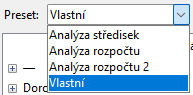
\includegraphics[width=1\textwidth]{presets_menu.png}
    \caption{Nabídka presetů}
    \label{fig:presets_menu}
\end{figure}
Po výběru presetu se hierarchie v záložce \textbf{Analýza} automaticky aktualizuje podle zvoleného presetu. Pokud zvolíme \textbf{Vlastní}, funkce \textbf{řádky} se odemkne a po kliknutí nám 
umožní ručně nastavovat hierarchii. Pomocí šipek nahoru a dolů můžeme měnit pořadí řádků, čímž měníme hierarchii zobrazenou v záložce \textbf{Analýza}. Pomocí šipek vlevo a vpravo můžeme volit, 
které řádky chceme zahrnout do hierarchie. (viz Obrázek \ref{fig:custom_rows}).
\begin{figure}[H]
    \centering
    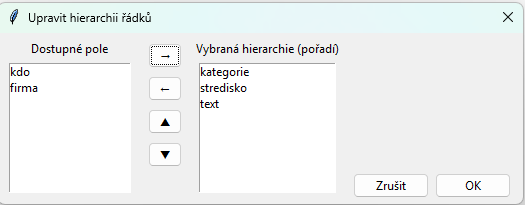
\includegraphics[width=1\textwidth]{custom_rows.png}
    \caption{Nastavení vlastních řádků pro hierarchii}
    \label{fig:custom_rows}
\end{figure}








\subsection{Dashboard}
Po splnění všech kroků tutoriálu se nám v záložce \textbf{Home} zobrazí kompletní dashboard, ten se ale může zobrazit v zamknutém stavu, pokud jsme ještě nenastavili rozpočet pro každou kategorii naší účetní osnovy 
(viz Obrázek \ref{fig:locked_dashboard}).
\begin{figure}[H]
    \centering
    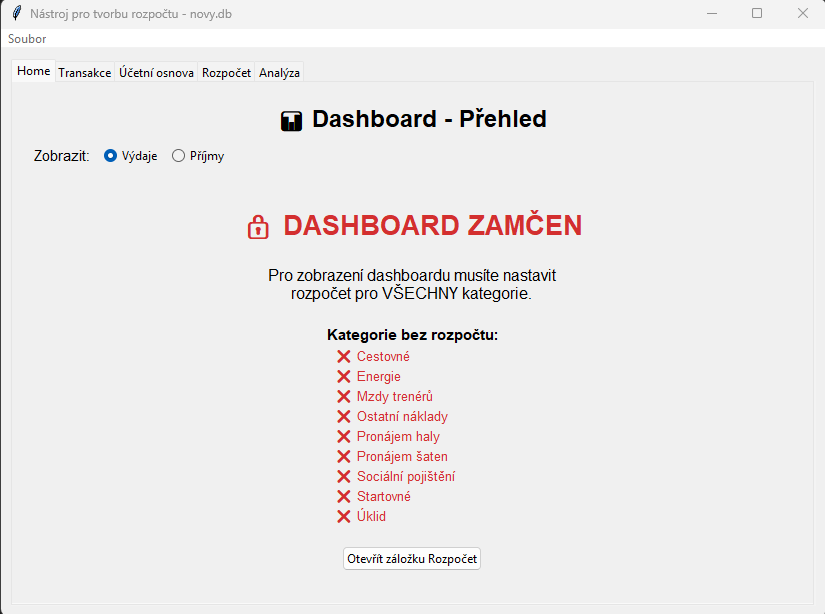
\includegraphics[width=1\textwidth]{locked_dashboard.png}
    \caption{Zamknutý dashboard}
    \label{fig:locked_dashboard}
\end{figure}
Pro odemčení dashboardu je potřeba nastavit rozpočet pro každou kategorii naší účetní osnovy. Po odemčení se nám zobrazí kompletní dashboard (viz Obrázek \ref{fig:complete_dashboard}).

\subsubsection{Hlavní přehled}
V dashboardu máme 2 hlavní sekce: \textbf{Výdaje} a \textbf{Příjmy} lze mezi nimi přepínat pomocí tlačítek v levé horní části (viz Obrázek \ref{fig:complete_dashboard}). 

Pod těmito tlačítky se nachází
jednotlivé měsíce, které zobrazujeme jako tlačítka pro rychlý přístup k datům daného měsíce. Na těchto tlačítkách vidíme \textbf{procentuální plnění rozpočtu YTD} (Year-To-Date, od začátku roku) pro daný měsíc a \textbf{Limit} ( očekávané plnění rozpočtu ((měsíc/12)*100)).

Jednotlivé tlačítka měsíců jsou barevně odlišena podle toho, zda YTD plnění rozpočtu je v limitu nebo jej překračuje:
\begin{itemize}
    \item \textbf{zelená barva} – YTD plnění rozpočtu je v limitu
    \item \textbf{žlutá barva} – YTD plnění rozpočtu překračuje limit, ale je v rozmezí 5\%
    \item \textbf{červená barva} – YTD plnění rozpočtu překračuje více než 5\%
\end{itemize}
\begin{figure}[H]
    \centering
    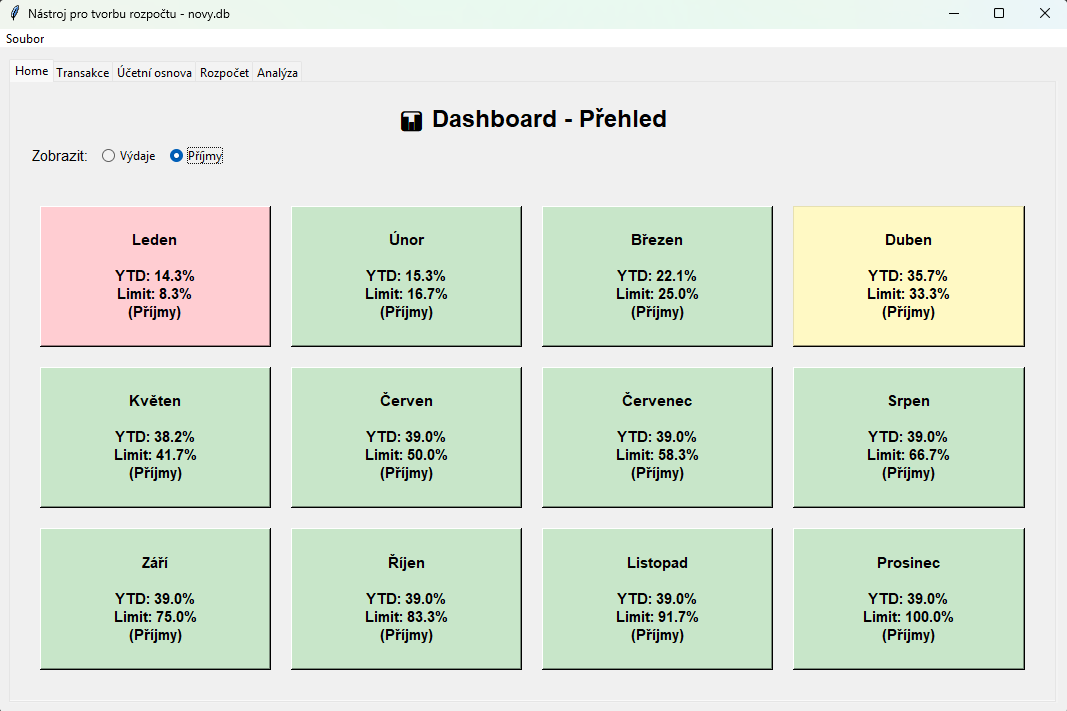
\includegraphics[width=1\textwidth]{complete_dashboard.png}
    \caption{Kompletní dashboard}
    \label{fig:complete_dashboard}
\end{figure}

Díky této logice můžeme vidět jak jsme na tom s plněním rozpočtu v jednotlivých měsících a můžeme se rychle dostat k detailní analýze daného měsíce kliknutím na tlačítko měsíce. Můžeme např. vidět, že v měsíci 
\textbf{Leden} máme plnění 14.4\% což je výrazně nad limitem 8.33\% a tlačítko je červené, proto můžeme kliknout na tlačítko \textbf{Leden} a podívat se na detailní analýzu tohoto měsíce 
(viz Obrázek \ref{fig:month_analysis}). 

\subsubsection{Měsíční analýza}
Po kliknutí na tlačítko měsíce se nám zobrazí podrobnější analýza daného měsíce (viz Obrázek \ref{fig:month_analysis}).
\begin{figure}[H]
    \centering
    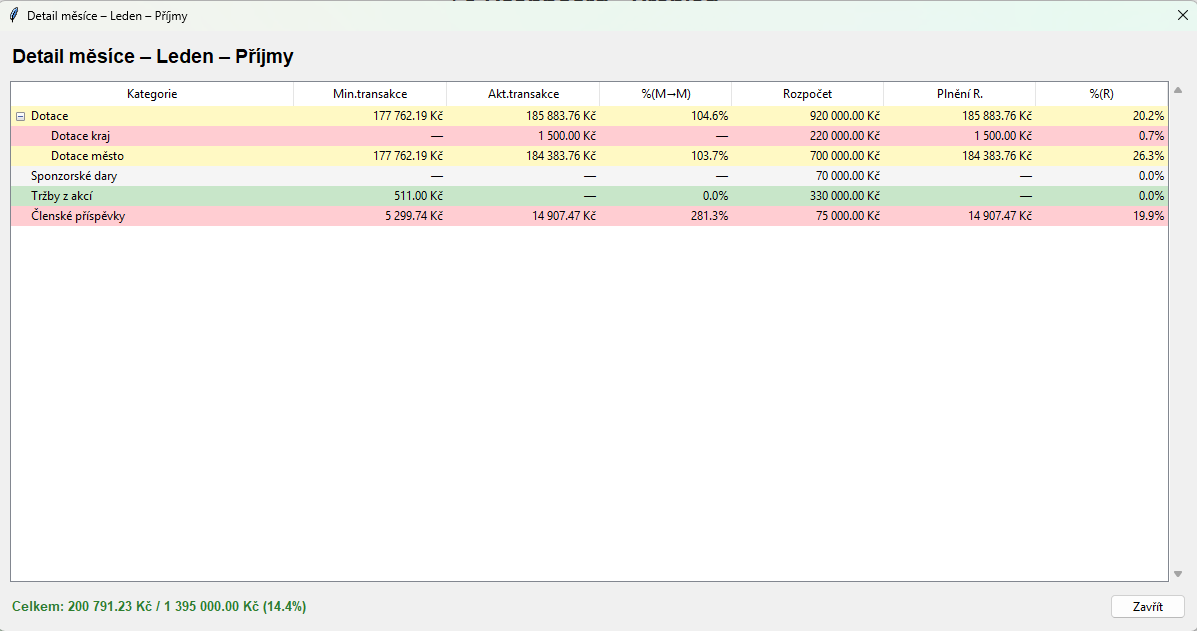
\includegraphics[width=1\textwidth]{month_analysis.png}
    \caption{Měsíční analýza}
    \label{fig:month_analysis}
\end{figure}
Na obrázku \ref{fig:month_analysis} vidíme opět naši hierarchii kategorií z účetní osnovy, ale tentokrát s podrobnějšími informacemi o daném měsíci.
Zobrazení hierarchie je stejné jako v záložce \textbf{Rozpočet}, ale máme zde nové sloupce:
\begin{itemize}
    \item \textbf{Min. transakce} – součet všech minulých transakcí v dané kategorii za vybraný měsíc.
    \item \textbf{Akt. transakce} – součet všech aktuálních transakcí v dané kategorii za vybraný měsíc.
    \item \textbf{\%(M->M)} – procentuální změna mezi minulými a aktuálními transakcemi za vybraný měsíc.
    \item \textbf{Rozpočet} – plánovaný rozpočet pro danou kategorii.
    \item \textbf{Plnění R.} – aktuální plnění rozpočtu pro danou kategorii YTD (Year-To-Date, od začátku roku).
    \item \textbf{\%(R)} – procentuální plnění rozpočtu pro danou kategorii YTD.
\end{itemize}
Zároveň dole vlevo vidíme hodnotu \textbf{Celkem}, tato hodnota zobrazuje plnění celkového rozpočtu YTD. Tuto hodnotu v \% můžeme vidět i na tlačítku měsíce v dashboardu (viz Obrázek \ref{fig:complete_dashboard}). 
V dashboardu se nám díky hodnotě \textbf{14.4\%} zobrazuje tlačítko červeně. Zde, ale vidíme, celkové plnění rozpočtu YTD a můžeme tak vyvodit, že i přes to, že jsme tento měsíc utratili více než je náš fixní limit, 
tak celkově jsme stále pod limitem v rámci rozpočtu a detailně vidíme přesnou částku. 

Je normální, že v některých měsících utratíme více a v jiných méně, důležité je sledovat celkové plnění rozpočtu v rámci roku. Díky této barevné logice můžeme identifikovat, které měsíce jsou více příjmové/výdajové 
a které méně.



\subsection{Záložka transakce}
Na obrázku \ref{fig:transactions_tab} vidíme záložku \textbf{Transakce}, která slouží k práci s aktuálními a historickými transakcemi. Zde můžeme vidět všechny transakce, které jsme importovali z excelu, případně 
přidali ručně. Mezi historické a aktuální transakce můžeme přepínat pomocí tlačítka textu \textbf{Přepnout na Historické/Aktuální transakce} v sekci pro akce s transakcemi (viz Obrázek \ref{fig:functions}).
\begin{figure}[H]
    \centering
    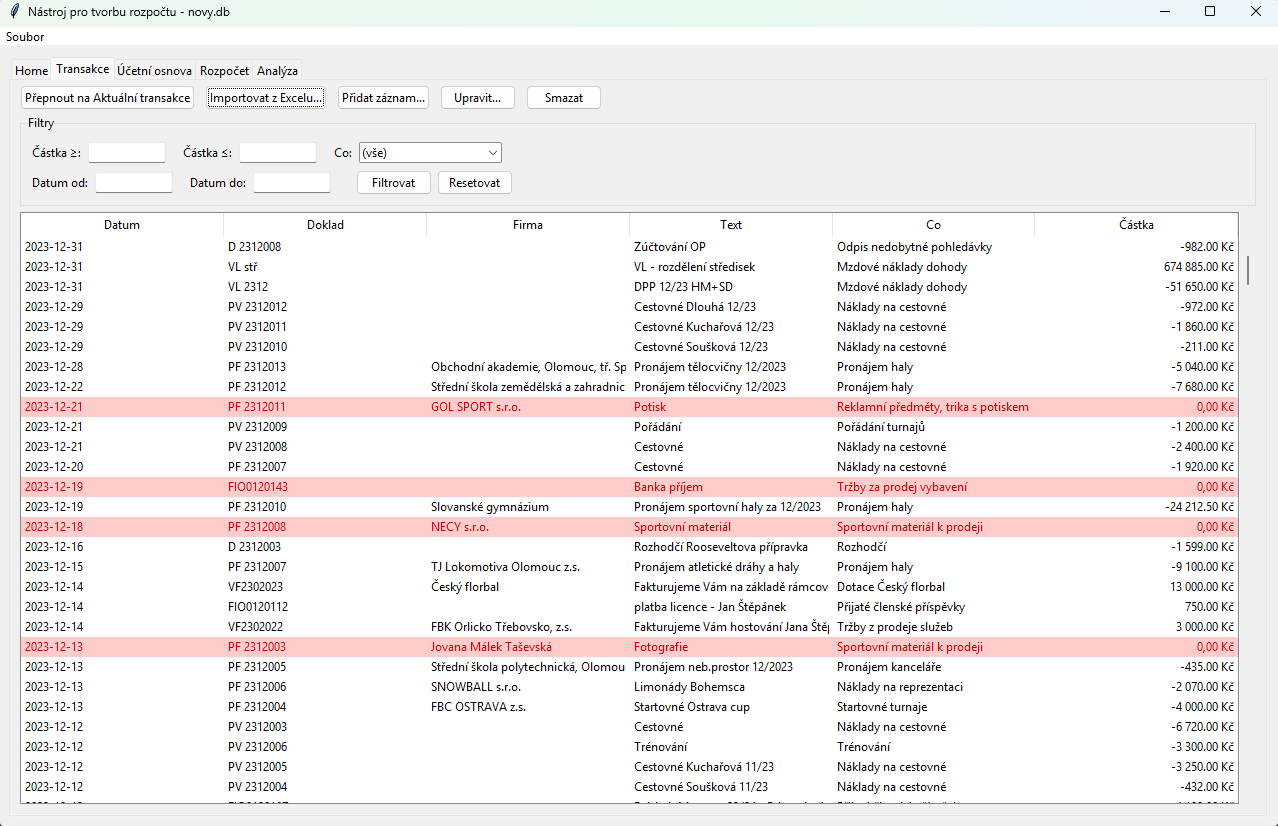
\includegraphics[width=1\textwidth]{transactions_tab.png}
    \caption{Záložka transakce}
    \label{fig:transactions_tab}
\end{figure}
\subsubsection{Vizualizace transakcí}
Jako první si můžeme na obrázku \ref{fig:transactions_tab} všimnout, že některé transakce jsou červené. To značí, že těmto transakcím chybí povinná položka buď text \textbf{Co} nebo \textbf{Částka}. Obě tyto 
položky jsou klíčové pro automatické určení kategorie a typu transakce. Pokud některá z těchto položek chybí, aplikace s touto transakcí nepracuje a je nutné ji opravit ručně (viz sekce Editace transakcí).

Při bližším pohledu si můžeme všimnout jednotlivých sloupců: \textbf{Datum}, \textbf{Doklad}, \textbf{Firma}, \textbf{Text}, \textbf{Co}, \textbf{Částka}.
Zobrazujeme pouze tyto sloupce z důvodu přehlednosti, ale aplikace interně uchovává všechny informace z excelu (případně z manuálně přidaných transakcí).Pokud chceme zobrazit více informací o dané transakci, 
můžeme na ni kliknout a poté kliknout na tlačítko \textbf{Upravit}, tím se nám zobrazí okno s kompletními informacemi o dané transakci (viz Obrázek \ref{fig:edit_transaction_window}).Tohle tlačítko slouží i 
pro editaci transakce (viz sekce Editace transakcí).
\subsubsection{Filtrování transakcí}
Aplikace umožňuje filtrovat transakce (viz Obrázek \ref{fig:filters}) podle částky (\textbf{částka >=} a \textbf{částka <=}), podle data (\textbf{Datum od} a \textbf{Datum do}) a podle kategorie (\textbf{Co} lze vybrat z rolldown menu
viz obrázek \ref{fig:rolldown}).
\begin{figure}[H]
    \centering
    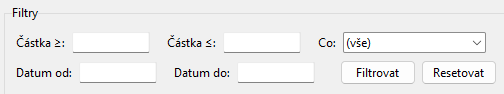
\includegraphics[width=1\textwidth]{filters.png}
    \caption{Filtrování transakcí}
    \label{fig:filters}
\end{figure} 
\begin{figure}[H]
    \centering
    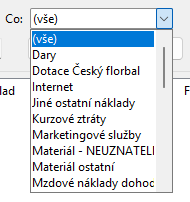
\includegraphics[width=0.5\textwidth]{rolldown.png}
    \caption{Rolldown menu pro výběr kategorie}
    \label{fig:rolldown}
\end{figure}
Tímto způsobem můžeme rychle najít konkrétní transakce, které nás zajímají. Po zadání požadovaných hodnot do filtrů je potřeba kliknout na tlačítko \textbf{Filtrovat}, tím se aktualizuje seznam transakcí podle 
zadaných kritérií. Filtry lze kombinovat a tím dosáhnout přesnějšího vyhledávání.

Pro resetování filtrů a zobrazení všech transakcí je potřeba kliknout na tlačítko \textbf{Resetovat}.
\subsubsection{Import transakcí}
Pro import nových transakcí můžeme využít tlačítko \textbf{Importovat z Excelu} nebo tlačítko \textbf{Přidat záznam}, které se nachází v sekci pro akce s transakcemi (viz Obrázek \ref{fig:functions}). 
Před importem/přidáním nových transakcí je potřeba zvolit, zda chceme pracovat s aktuálními nebo historickými transakcemi, podle toho se nám pak nové transakce zařadí. (viz sekce Založka transakce).
\begin{figure}[H]
    \centering
    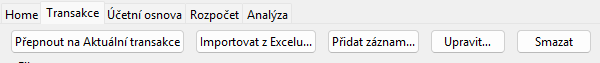
\includegraphics[width=1\textwidth]{functions.png}
    \caption{Sekce pro akce s transakcemi}
    \label{fig:functions}
\end{figure}
Při kliknutí na tlačítko \textbf{Importovat z Excelu} se zobrazí dialogové okno pro výběr souboru (viz Obrázek \ref{fig:choose_window}). Pro import je potřeba mít připravený excelový soubor, který obsahuje list s názvem \textbf{Zdroj}.
Tento list musí obsahovat sloupce: \textbf{Datum, Doklad, Zdroj, Firma, Text, MD, D, částka, Cin, číslo, Co, Kdo, Středisko}. Po výběru souboru se nás ještě aplikace dotáže, zda chceme přidat nové transakce k
existujícím nebo je nahradit (viz Obrázek \ref{fig:import_options}).
\begin{figure}[H]
    \centering
    
\includegraphics[width=0.8\textwidth]{import_options.png}
    \caption{Možnosti importu transakcí}
    \label{fig:import_options}
\end{figure}
Po potvrzení importu se nám zobrazí potvrzení importu a data se zařadí.

Při kliknutí na tlačítko \textbf{Přidat záznam} se zobrazí okno pro manuální přidání nové transakce (viz Obrázek \ref{fig:add_transaction_window}).
\begin{figure}[H]
    \centering
    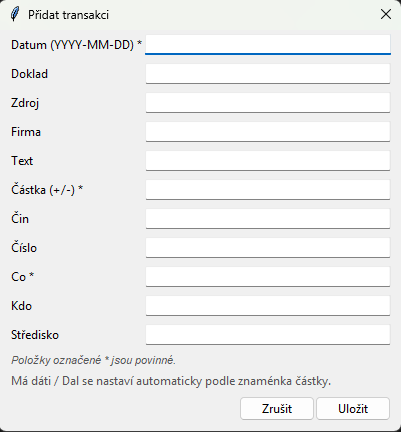
\includegraphics[width=0.8\textwidth]{add_transaction_window.png}
    \caption{Okno pro přidání nové transakce}
    \label{fig:add_transaction_window}
\end{figure}
Uživatel vyplní požadované informace o transakci a klikne na tlačítko \textbf{Uložit}, tím se nová transakce přidá do seznamu. Nutné položky \textbf{Datum}, \textbf{Co} a \textbf{Částka} jsou označeny hvězdičkou (*). O MD/D 
se aplikace postará sama na základě hodnoty v částce (kladná/ záporná).

Aplikace po přidání nové transakce automaticky určí kategorii a typ transakce na základě hodnot v poli \textbf{Co} a \textbf{Částka}. Pokud kategorie neexistuje v účetní osnově, transakce zůstane nezařazená 
a je potřeba ji zařadit ručně (viz sekce Tvorba osnovy).

\subsubsection{Editace transakcí}
Pro editaci existující transakce je potřeba ji nejdříve vybrat v seznamu a poté kliknout na tlačítko \textbf{Upravit} (viz Obrázek \ref{fig:functions}). Tím se nám zobrazí okno pro úpravu transakce 
(viz Obrázek \ref{fig:edit_transaction_window}).
Uživatel může upravit požadované
\begin{figure}[H]
    \centering
    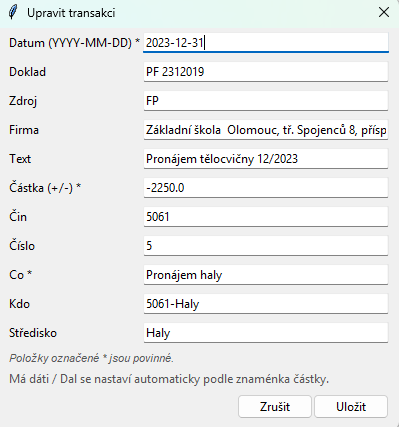
\includegraphics[width=0.8\textwidth]{edit_transaction_window.png}
    \caption{Okno pro úpravu transakce}
    \label{fig:edit_transaction_window}
\end{figure}
Editování transakcí je obdobné jako přidávání nových transakcí, uživatel může změnit jakékoliv pole a poté kliknout na tlačítko \textbf{Uložit} pro uložení změn. Nutné položky \textbf{Datum}, \textbf{Co} 
a \textbf{Částka} jsou označeny hvězdičkou (*). O MD/D se aplikace postará sama na základě hodnoty v částce (kladná/ záporná).

Aplikace po uložení změn automaticky aktualizuje kategorii a typ transakce na základě nových hodnot v poli \textbf{Co} a \textbf{Částka}. účetní osnova a rozpočet se tímto nijak neovlivní, pouze se změní zařazení dané 
transakce.
\subsubsection{Mazání transakcí}
Pro smazání transakce je potřeba ji nejdříve vybrat v seznamu a poté kliknout na tlačítko \textbf{Smazat} (viz Obrázek \ref{fig:functions}). Aplikace se nás ještě zeptá na potvrzení smazání 
(viz Obrázek \ref{fig:delete_confirm}).
\begin{figure}[H]
    \centering
    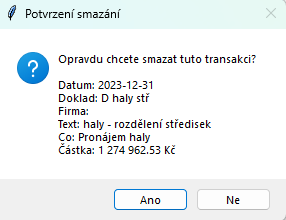
\includegraphics[width=0.8\textwidth]{delete_confirm.png}
    \caption{Potvrzení smazání transakce}
    \label{fig:delete_confirm}
\end{figure}
Po potvrzení se vybraná transakce smaže ze seznamu. Mazání transakcí nám neovlivňuje účetní osnovu ani rozpočet, pouze se odstraní z historie transakcí (ovlivní tedy pouze dashboard, 
pokud je daná transakce součástí účetní osnovy).

%% Povinné závěry
\begin{kiconclusions}
V této bakalářské práci byla navržena a implementována aplikace pro tvorbu a správu rozpočtů. Aplikace splňuje všechny stanovené požadavky...
\end{kiconclusions}

%% Přílohy
\appendix

\section{Obsah přiloženého média}
\begin{itemize}
    \item Zdrojové kódy aplikace
    \item Text práce ve formátu PDF
    \item Instalační soubory
\end{itemize}

\end{document}
